\newcommand{\hsmasprache}{en} 

% Dokumententyp und benutzte Pakete
\documentclass[open=right,  % Kapitel darf nur auf rechten Seite beginnen
    paper=a4,               % DIN-A4-Papier
    fontsize=12pt,          % Schriftgöße
    headings=small,         % Kleine Überschriften
    headsepline=true,       % Trennlinie am Kopf der Seite
    footsepline=false,      % Keine Trennlinie am Fuß der Seite
    bibliography=totoc,     % Literaturverzeichnis in das Inhaltsverzeichnis aufnehmen
    twoside=on,             % Doppelseitiger Druck - auf off stellen für einseitig
    DIV=7,                  % Verhältnis der Ränder zum bedruckten Bereich
    chapterprefix=true,     % Kapitel x vor dem Kapitelnamen
    cleardoublepage=plain]{scrbook}

% Pakete einbinden, die benötigt werden
\usepackage{ifthen}               % Logische Bedingungen mit ifthenelse
\usepackage{scrlayer-scrpage}
\usepackage[utf8]{inputenc}       % Dateien in UTF-8 benutzen
\usepackage[T1]{fontenc}          % Zeichenkodierung
\usepackage{graphicx}             % Bilder einbinden
\usepackage{enumitem}             % Eigene Listen definieren können

% Setzen von Optionen abhängig von der gewählten Sprache. Die Sprache wird
% in thesis.tex gesetzt.
\ifthenelse{\equal{\hsmasprache}{de}}%
  {%
   \usepackage[main=ngerman, english]{babel}  % Deutsche Sprachunterstützung
   \usepackage[autostyle=true,german=quotes]{csquotes} % Deutsche Anführungszeichen
   \usepackage[pagebackref=false,german]{hyperref} % Hyperlinks
   \newcommand{\hsmasortlocale}{de_DE} % Sortierung der Literatur
  }%
  {%
   \usepackage[main=english, ngerman]{babel} % Englische Sprachunterstützung
   \usepackage[autostyle=true,english=american]{csquotes} % Englische Anführungszeichen
   \usepackage[pagebackref=false,english]{hyperref}  % Hyperlinks
   \newcommand{\hsmasortlocale}{en_US} % Sortierung der Literatur
  }%
\usepackage[table]{xcolor}% http://ctan.org/pkg/xcolor
\usepackage{xcolor}               % Unterstützung für Farben
\usepackage{amsmath}              % Mathematische Formeln
\usepackage{amsfonts}             % Mathematische Zeichensätze
\usepackage{amssymb}              % Mathematische Symbole
\usepackage{float}                % Fließende Objekte (Tabellen, Grafiken etc.)
\usepackage{makecell}
\usepackage{booktabs}             % Korrekter Tabellensatz
\usepackage[printonlyused]{acronym}  % Abkürzungsverzeichnis [nur verwendete Abkürzungen]
\usepackage{makeidx}              % Sachregister
\usepackage{listings}             % Quelltexte
\usepackage{listingsutf8}         % Quelltexte in UTF8
\usepackage[hang,font={sf,footnotesize},labelfont={footnotesize,bf}]{caption} % Beschriftungen
\usepackage[scaled]{helvet}       % Schrift Helvetia laden
\usepackage[absolute]{textpos}    % Absolute Textpositionen (für Deckblatt)
\usepackage{calc}                 % Berechnung von Positionen
\usepackage{blindtext}            % Blindtexte
\usepackage[bottom=40mm,left=35mm,right=35mm,top=30mm]{geometry} % Ränder ändern
\usepackage{setspace}             % Abstände korrigieren
\usepackage{scrhack}              % tocbasic Warnung entfernen
\usepackage[all]{hypcap}          % Korrekte Verlinkung von Floats
\usepackage{tabularx}             % Spezielle Tabellen
\usepackage[backend=biber,
  isbn=false,                     % ISBN nicht anzeigen, gleiches geht mit nahezu allen anderen Feldern
  sortlocale=en_EN,     % Sortierung der Einträge für Deutsch
                                  %      de_DE: für Deutsch
                                  %      en_US: für Englisch
  autocite=inline,                % regelt Aussehen für \autocite
                                  %      inline: Zitat in Klammern (\parancite)
                                  %      footnote: Zitat in Fußnoten (\footcite)
                                  %      plain: Zitat direkt ohne Klammern (\cite)
  style=numeric,               % Legt den Stil für die Zitate fest
                                  %      ieee: Zitate als Zahlen [1]
                                  %      alphabetic: Zitate als Kürzel und Jahr [Ein05]
                                  %      authoryear: Zitate Author und Jahr [Einstein (1905)]
  hyperref=true,                  % Hyperlinks für Zitate
  citestyle=numeric,
  firstinits=false                % Vornamen abkürzen (Maier, M. anstatt Maier, Markus)?
                                  %      true: abkürzen
                                  %      false: nicht abkürzen
]{biblatex}                       % Literaturverwaltung mit BibLaTeX
\usepackage{rotating}             % Seiten drehen
\usepackage{harveyballs}          % Harveyballs
\usepackage{chngcntr}             % Counter (Zähler) ändern können - für Fußnotennummern

% Einstellungen zu den Fußnoten
\renewcommand{\footnotesize}{\fontsize{9}{10}\selectfont} % Größe der Fußnoten
\setlength{\footnotesep}{8pt} % Abstand zwischen den Fußnoten

% Kommentieren Sie diese Zeile ein, wenn Sie eine "durchlaufende" Nummerierung bei den
% Fußnoten wünschen, d.h. wenn die Fußnoten nicht bei jedem Kapitel wieder bei 1
% beginnen sollen.
%\counterwithout{footnote}{chapter}

\setlength{\bibitemsep}{1em}      % Abstand zwischen den Literaturangaben
\setlength{\bibhang}{2em}         % Einzug nach jeweils erster Zeile

% Trennung von URLs im Literaturverzeichnis (große Werte [> 10000] verhindern die Trennung)
\defcounter{biburlnumpenalty}{10} % Strafe für Trennung in URL nach Zahl
\defcounter{biburlucpenalty}{500} % Strafe für Trennung in URL nach Großbuchstaben
\defcounter{biburllcpenalty}{500} % Strafe für Trennung in URL nach Kleinbuchstaben

% Farben definieren
\definecolor{linkblue}{RGB}{0, 0, 100}
\definecolor{linkblack}{RGB}{0, 0, 0}
\definecolor{comment}{RGB}{63, 127, 95}
\definecolor{darkgreen}{RGB}{14, 144, 102}
\definecolor{darkblue}{RGB}{0,0,168}
\definecolor{darkred}{RGB}{128,0,0}
\definecolor{javadoccomment}{RGB}{0,0,240}

% Einstellungen für das Hyperlink-Paket
\hypersetup{
    colorlinks=true,      % Farbige links verwenden
%    allcolors=linkblue,
    linktoc=all,          % Links im Inhaltsverzeichnis
    linkcolor=linkblack,  % Querverweise
    citecolor=linkblack,  % Literaturangaben
    filecolor=linkblack,  % Dateilinks
    urlcolor=linkblack    % URLs
}

% Einstellungen für Quelltexte
\lstset{
      xleftmargin=0.2cm,
      basicstyle=\footnotesize\ttfamily,
      keywordstyle=\color{darkgreen},
      identifierstyle=\color{darkblue},
      commentstyle=\color{comment},
      stringstyle=\color{darkred},
      tabsize=2,
      lineskip={2pt},
      columns=flexible,
      inputencoding=utf8,
      captionpos=b,
      breakautoindent=true,
      breakindent=2em,
      breaklines=true,
      prebreak=,
      postbreak=,
      numbers=none,
      numberstyle=\tiny,
      showspaces=false,      % Keine Leerzeichensymbole
      showtabs=false,        % Keine Tabsymbole
      showstringspaces=false,% Leerzeichen in Strings
      morecomment=[s][\color{javadoccomment}]{/**}{*/},
      literate={Ö}{{\"O}}1 {Ä}{{\"A}}1 {Ü}{{\"U}}1 {ß}{{\ss}}2 {ü}{{\"u}}1 {ä}{{\"a}}1 {ö}{{\"o}}1
}

\urlstyle{same}

% Einstellungen für Überschriften
\renewcommand*{\chapterformat}{%
  \Large\chapapp~\thechapter   % Große Schrift
  \vspace{0.3cm}               % Abstand zum Titel des Kapitels
}

% Abstände für die Überschriften setzen
\renewcommand{\chapterheadstartvskip}{\vspace*{2.6cm}}
\renewcommand{\chapterheadendvskip}{\vspace*{1.5cm}}

% Vertikale Abstände für die Überschriften etwas verkleinern
\RedeclareSectionCommand[
  beforeskip=-1.8\baselineskip,
  afterskip=0.25\baselineskip]{section}

\RedeclareSectionCommand[
  beforeskip=-1.8\baselineskip,
  afterskip=0.15\baselineskip]{subsection}

\RedeclareSectionCommand[
  beforeskip=-1.8\baselineskip,
  afterskip=0.15\baselineskip]{subsubsection}

% In der Kopfzeile nur die kurze Kapitelbezeichnung (ohne Kapitel davor)
\renewcommand*\chaptermarkformat{\thechapter\autodot\enskip}
\automark[chapter]{chapter}

% Einstellungen für Schriftarten
\setkomafont{pagehead}{\normalfont\sffamily}
\setkomafont{pagenumber}{\normalfont\sffamily}
\setkomafont{paragraph}{\sffamily\bfseries\small}
\setkomafont{subsubsection}{\sffamily\itshape\bfseries\small}
\addtokomafont{footnote}{\footnotesize}
\setkomafont{chapter}{\LARGE\selectfont\bfseries}

% Wichtige Abstände
\setlength{\parskip}{0.2cm}  % 2mm Abstand zwischen zwei Absätzen
\setlength{\parindent}{0mm}  % Absätze nicht einziehen
\clubpenalty = 10000         % Keine "Schusterjungen"
\widowpenalty = 10000        % Keine "Hurenkinder"
\displaywidowpenalty = 10000 % Keine "Hurenkinder"
                             % Siehe: https://de.wikipedia.org/wiki/Hurenkind_und_Schusterjunge

% Index erzeugen
\makeindex

% Einfacher Font-Wechsel über dieses Makro
\newcommand{\changefont}[3]{
\fontfamily{#1} \fontseries{#2} \fontshape{#3} \selectfont}

% Eigenes Makro für Bilder. Das label (für \ref) ist dann einfach
% der Name der Bilddatei
\newcommand{\bild}[3]{
\begin{figure}[ht]
  \centering
  \includegraphics[width=#2]{#1}
  \caption{#3}
  \label{#1}
\end{figure}}

% Wo liegt Sourcecode?
\newcommand{\srcloc}{src/}

% Wo sind die Bilder?
\graphicspath{{bilder/}}

% Makros für typographisch korrekte Abkürzungen
\newcommand{\zb}[0]{z.\,B.}
\newcommand{\dahe}[0]{d.\,h.}
\newcommand{\ua}[0]{u.\,a.}

% Flags für Veröffentlichung und Sperrvermerk
\newboolean{hsmapublizieren}
\newboolean{hsmasperrvermerk}

% Tabellenzellen mit mehreren Zeilen
\newcolumntype{L}{>{\raggedright\arraybackslash}X}
\newcolumntype{b}{l}
\newcolumntype{s}{>{\hsize=.3\hsize}l}
\newcolumntype{F}{>{\hsize=\dimexpr2\hsize+2\tabcolsep+\arrayrulewidth\relax}X}

% Checklisten mit zwei Ebenen
\newlist{checklist}{itemize}{2}
\setlist[checklist]{label=$\square$}

% -------------------------------------------------------
% Daten für die Arbeit
% Wenn hier alles korrekt eingetragen wurde, wird das Titelblatt
% automatisch generiert. D.h. die Datei titelblatt.tex muss nicht mehr
% angepasst werden.

% Titel der Arbeit auf Deutsch
\newcommand{\hsmatitelde}{Konzeption, Implementierung und Bewertung eines modularen Proxys zum Testen von Anwendungen im Internet der Dinge}

% Titel der Arbeit auf Englisch
\newcommand{\hsmatitelen}{Conception, Implementation and Evaluation of a Modular Proxy Application for Testing Internet of Things Applications}

% Weitere Informationen zur Arbeit
\newcommand{\hsmaort}{Mannheim}    % Ort
\newcommand{\hsmaautorvname}{Moritz Laurin} % Vorname(n)
\newcommand{\hsmaautornname}{Thomas} % Nachname(n)
\newcommand{\hsmadatum}{31.03.2021} % Datum der Abgabe
\newcommand{\hsmajahr}{2020} % Jahr der Abgabe
\newcommand{\hsmafirma}{NVISO GmbH, Frankfurt} % Firma bei der die Arbeit durchgeführt wurde
\newcommand{\hsmabetreuer}{Prof. Dr. Thomas Specht, Hochschule Mannheim} % Betreuer an der Hochschule
\newcommand{\hsmazweitkorrektor}{Pierre-Alain Mouy, M.Sc., NVISO GmbH} % Betreuer im Unternehmen oder Zweitkorrektor
\newcommand{\hsmafakultaet}{I} % I für Informatik oder E, S, B, D, M, N, W, V
\newcommand{\hsmastudiengang}{IM} % IB IMB UIB CSB IM MTB (weitere siehe titleblatt.tex)

% Zustimmung zur Veröffentlichung
\setboolean{hsmapublizieren}{true}   % Einer Veröffentlichung wird zugestimmt
\setboolean{hsmasperrvermerk}{false} % Die Arbeit hat keinen Sperrvermerk

% -------------------------------------------------------
% Abstract
% Achtung: Wenn Sie im Abstrakt Anführungszeichen verwenden wollen, dann benutzen Sie
%          nicht "` und "', sondern \enquote{}. "` und "' werden nicht richtig
%          erkannt.

% Kurze (maximal halbseitige) Beschreibung, worum es in der Arbeit geht auf Deutsch
\newcommand{\hsmaabstractde}{TBD.} % TODO

% Kurze (maximal halbseitige) Beschreibung, worum es in der Arbeit geht auf Englisch
\newcommand{\hsmaabstracten}{TBD} %TODO


\addbibresource{literature.bib}   

\begin{document}
\frontmatter

\setcounter{page}{0}
\changefont{ptm}{m}{n}  
\renewcommand{\rmdefault}{ptm}

% *******************************************************************
% In dieser Datei sollten eigentlich keine Veränderungen
% notwendig sein. Alle Einstellungen erfolgen in docinfo.tex und
% der thesis.tex.
% *******************************************************************

\thispagestyle{empty}

% Fakultäten der HS-Mannheim
% *******************************************************************
\ifthenelse{\equal{\hsmafakultaet}{I}}%
  {\newcommand{\hsmafakultaetlangde}{Fakultät für Informatik}%
   \newcommand{\hsmafakultaetlangen}{Department of Computer Science}}{}

\ifthenelse{\equal{\hsmafakultaet}{E}}%
  {\newcommand{\hsmafakultaetlangde}{Fakultät für Elektrotechnik}%
   \newcommand{\hsmafakultaetlangen}{Department of Electrical Engineering}}{}

\ifthenelse{\equal{\hsmafakultaet}{S}}%
  {\newcommand{\hsmafakultaetlangde}{Fakultät für Sozialwesen}%
   \newcommand{\hsmafakultaetlangen}{Department of Social Work}}{}

\ifthenelse{\equal{\hsmafakultaet}{B}}%
  {\newcommand{\hsmafakultaetlangde}{Fakultät für Biotechnologie}%
   \newcommand{\hsmafakultaetlangen}{Department of Biotechnology}}{}

\ifthenelse{\equal{\hsmafakultaet}{D}}%
  {\newcommand{\hsmafakultaetlangde}{Fakultät für Gestaltung}%
   \newcommand{\hsmafakultaetlangen}{Department of Design}}{}

\ifthenelse{\equal{\hsmafakultaet}{M}}%
  {\newcommand{\hsmafakultaetlangde}{Fakultät für Maschinenbau}%
   \newcommand{\hsmafakultaetlangen}{Department of Mechanical Engineering}}{}

\ifthenelse{\equal{\hsmafakultaet}{N}}%
  {\newcommand{\hsmafakultaetlangde}{Fakultät für Informationstechnik}%
   \newcommand{\hsmafakultaetlangen}{Department of Information Technology}}{}

\ifthenelse{\equal{\hsmafakultaet}{W}}%
  {\newcommand{\hsmafakultaetlangde}{Fakultät für Wirtschaftsingenieurwesen}%
   \newcommand{\hsmafakultaetlangen}{Department of Engineering and Management}}{}

\ifthenelse{\equal{\hsmafakultaet}{V}}%
  {\newcommand{\hsmafakultaetlangde}{Fakultät für Verfahrens- und Chemietechnik}%
   \newcommand{\hsmafakultaetlangen}{Department of Chemical Process Engineering}}{}

% Studiengänge der HS-Mannheim
% *******************************************************************
\ifthenelse{\equal{\hsmastudiengang}{IB}}%
  {\newcommand{\hsmastudienganglangde}{Informatik}%
  \newcommand{\hsmastudienganglangen}{Computer Science}%
  \newcommand{\hsmatypde}{Bachelor-Thesis}%
  \newcommand{\hsmatypen}{Bachelor Thesis}%
  \newcommand{\hsmagrad}{\hsmabsc}}{}

\ifthenelse{\equal{\hsmastudiengang}{IMB}}%
  {\newcommand{\hsmastudienganglangde}{Medizinische Informatik}%
  \newcommand{\hsmastudienganglangen}{Medical Informatics}%
  \newcommand{\hsmatypde}{Bachelor-Thesis}%
  \newcommand{\hsmatypen}{Bachelor Thesis}%
  \newcommand{\hsmagrad}{\hsmabsc}}{}

\ifthenelse{\equal{\hsmastudiengang}{UIB}}%
  {\newcommand{\hsmastudienganglangde}{Unternehmens- und Wirtschaftsinformatik}%
  \newcommand{\hsmastudienganglangen}{Enterprise Computing}%
  \newcommand{\hsmatypde}{Bachelor-Thesis}%
  \newcommand{\hsmatypen}{Bachelor Thesis}%
  \newcommand{\hsmagrad}{\hsmabsc}}{}

\ifthenelse{\equal{\hsmastudiengang}{CSB}}%
  {\newcommand{\hsmastudienganglangde}{Cyber Security}%
  \newcommand{\hsmastudienganglangen}{Cyber Security}%
  \newcommand{\hsmatypde}{Bachelor-Thesis}%
  \newcommand{\hsmatypen}{Bachelor Thesis}%
  \newcommand{\hsmagrad}{\hsmabsc}}{}

\ifthenelse{\equal{\hsmastudiengang}{IM}}%
  {\newcommand{\hsmastudienganglangde}{Informatik}%
   \newcommand{\hsmastudienganglangen}{Computer Science}%
   \newcommand{\hsmatypde}{Master-Thesis}%
   \newcommand{\hsmatypen}{Master Thesis}%
   \newcommand{\hsmagrad}{\hsmamaster}}{}

\ifthenelse{\equal{\hsmastudiengang}{MEB}}%
  {\newcommand{\hsmastudienganglangde}{Mechatronik}%
   \newcommand{\hsmastudienganglangen}{Mechatronic}%
   \newcommand{\hsmatypde}{Bachelor-Thesis}%
   \newcommand{\hsmatypen}{Bachelor Thesis}%
   \newcommand{\hsmagrad}{\hsmabsc}}{}

\ifthenelse{\equal{\hsmastudiengang}{UB}}%
  {\newcommand{\hsmastudienganglangde}{Automatisierungstechnik}%
   \newcommand{\hsmastudienganglangen}{Automation Technology}%
   \newcommand{\hsmatypde}{Bachelor-Thesis}%
   \newcommand{\hsmatypen}{Bachelor Thesis}%
   \newcommand{\hsmagrad}{\hsmabsc}}{}

\ifthenelse{\equal{\hsmastudiengang}{ELB}}%
  {\newcommand{\hsmastudienganglangde}{Elektro- und Informationstechnik/Ingenieurpädagogik}%
   \newcommand{\hsmastudienganglangen}{Elektro- und Informationstechnik/Ingenieurpädagogik}%
   \newcommand{\hsmatypde}{Bachelor-Thesis}%
   \newcommand{\hsmatypen}{Bachelor Thesis}%
   \newcommand{\hsmagrad}{\hsmabsc}}{}

\ifthenelse{\equal{\hsmastudiengang}{EBE}}%
  {\newcommand{\hsmastudienganglangde}{Energietechnik und erneuerbare Energien}%
   \newcommand{\hsmastudienganglangen}{Power Engineering ans Renewable Energies}%
   \newcommand{\hsmatypde}{Bachelor-Thesis}%
   \newcommand{\hsmatypen}{Bachelor Thesis}%
   \newcommand{\hsmagrad}{\hsmabsc}}{}

\ifthenelse{\equal{\hsmastudiengang}{TS}}%
  {\newcommand{\hsmastudienganglangde}{Translation Studies}%
   \newcommand{\hsmastudienganglangen}{Translation Studies}%
   \newcommand{\hsmatypde}{Bachelor-Thesis}%
   \newcommand{\hsmatypen}{Bachelor Thesis}%
   \newcommand{\hsmagrad}{\hsmabsc}}{}

\ifthenelse{\equal{\hsmastudiengang}{EM}}%
  {\newcommand{\hsmastudienganglangde}{Automatisierungs- und Energiesysteme}%
   \newcommand{\hsmastudienganglangen}{Automation and Energy Systems}%
   \newcommand{\hsmatypde}{Master-Thesis}%
   \newcommand{\hsmatypen}{Master Thesis}%
   \newcommand{\hsmagrad}{\hsmamaster}}{}

\ifthenelse{\equal{\hsmastudiengang}{ELM}}%
  {\newcommand{\hsmastudienganglangde}{Lehramt Ingenieurpädagogik}%
   \newcommand{\hsmastudienganglangen}{Lectureship Educational Engineering}%
   \newcommand{\hsmatypde}{Master-Thesis}%
   \newcommand{\hsmatypen}{Master Thesis}%
   \newcommand{\hsmagrad}{\hsmamaster}}{}

\ifthenelse{\equal{\hsmastudiengang}{SAB}}%
  {\newcommand{\hsmastudienganglangde}{Soziale Arbeit}%
   \newcommand{\hsmastudienganglangen}{Social Labour}%
   \newcommand{\hsmatypde}{Bachelor-Thesis}%
   \newcommand{\hsmatypen}{Bachelor Thesis}%
   \newcommand{\hsmagrad}{\hsmaba}}{}

\ifthenelse{\equal{\hsmastudiengang}{SAM}}%
  {\newcommand{\hsmastudienganglangde}{Soziale Arbeit}%
   \newcommand{\hsmastudienganglangen}{Social Labour}%
   \newcommand{\hsmatypde}{Master-Thesis}%
   \newcommand{\hsmatypen}{Master Thesis}%
   \newcommand{\hsmagrad}{\hsmamastera}}{}

\ifthenelse{\equal{\hsmastudiengang}{BB}}%
  {\newcommand{\hsmastudienganglangde}{Biotechnology}%
   \newcommand{\hsmastudienganglangen}{Biotechnology}%
   \newcommand{\hsmatypde}{Bachelor-Thesis}%
   \newcommand{\hsmatypen}{Bachelor Thesis}%
   \newcommand{\hsmagrad}{\hsmabsc}}{}

\ifthenelse{\equal{\hsmastudiengang}{BCB}}%
  {\newcommand{\hsmastudienganglangde}{Biologische Chemie}%
   \newcommand{\hsmastudienganglangen}{Biological Chemics}%
   \newcommand{\hsmatypde}{Bachelor-Thesis}%
   \newcommand{\hsmatypen}{Bachelor Thesis}%
   \newcommand{\hsmagrad}{\hsmabsc}}{}

\ifthenelse{\equal{\hsmastudiengang}{BMEBST}}%
  {\newcommand{\hsmastudienganglangde}{Biotechnology - Biomedical Science and Technology}%
   \newcommand{\hsmastudienganglangen}{Biotechnology - Biomedical Science and Technology}%
   \newcommand{\hsmatypde}{Master-Thesis}%
   \newcommand{\hsmatypen}{Master Thesis}%
   \newcommand{\hsmagrad}{\hsmamaster}}{}

\ifthenelse{\equal{\hsmastudiengang}{BMEBPD}}%
  {\newcommand{\hsmastudienganglangde}{Biotechnology - Bioprocess Development}%
   \newcommand{\hsmastudienganglangen}{Biotechnology - Bioprocess Development}%
   \newcommand{\hsmatypde}{Master-Thesis}%
   \newcommand{\hsmatypen}{Master Thesis}%
   \newcommand{\hsmagrad}{\hsmamaster}}{}

\ifthenelse{\equal{\hsmastudiengang}{BLSM}}%
  {\newcommand{\hsmastudienganglangde}{Life Science Management}%
   \newcommand{\hsmastudienganglangen}{Life Science Management}%
   \newcommand{\hsmatypde}{Master-Thesis}%
   \newcommand{\hsmatypen}{Master Thesis}%
   \newcommand{\hsmagrad}{\hsmamaster}}{}

\ifthenelse{\equal{\hsmastudiengang}{KDB}}%
  {\newcommand{\hsmastudienganglangde}{Kommunikationsdesign}%
   \newcommand{\hsmastudienganglangen}{Communication Design}%
   \newcommand{\hsmatypde}{Bachelor-Thesis}%
   \newcommand{\hsmatypen}{Bachelor Thesis}%
   \newcommand{\hsmagrad}{\hsmaba}}{}

\ifthenelse{\equal{\hsmastudiengang}{KDM}}%
  {\newcommand{\hsmastudienganglangde}{Kommunikationsdesign}%
   \newcommand{\hsmastudienganglangen}{Communication Design}%
   \newcommand{\hsmatypde}{Master-Thesis}%
   \newcommand{\hsmatypen}{Master Thesis}%
   \newcommand{\hsmagrad}{\hsmamastera}}{}

\ifthenelse{\equal{\hsmastudiengang}{MB}}%
  {\newcommand{\hsmastudienganglangde}{Maschinenbau}%
   \newcommand{\hsmastudienganglangen}{Mechanical Engineering}%
   \newcommand{\hsmatypde}{Bachelor-Thesis}%
   \newcommand{\hsmatypen}{Bachelor Thesis}%
   \newcommand{\hsmagrad}{\hsmabsc}}{}

\ifthenelse{\equal{\hsmastudiengang}{MM}}%
  {\newcommand{\hsmastudienganglangde}{Maschinenbau}%
   \newcommand{\hsmastudienganglangen}{Mechanical Engineering}%
   \newcommand{\hsmatypde}{Master-Thesis}%
   \newcommand{\hsmatypen}{Master Thesis}%
   \newcommand{\hsmagrad}{\hsmamaster}}{}

\ifthenelse{\equal{\hsmastudiengang}{NEB}}%
  {\newcommand{\hsmastudienganglangde}{Elektronik}%
   \newcommand{\hsmastudienganglangen}{Electronics}%
   \newcommand{\hsmatypde}{Bachelor-Thesis}%
   \newcommand{\hsmatypen}{Bachelor Thesis}%
   \newcommand{\hsmagrad}{\hsmabsc}}{}

\ifthenelse{\equal{\hsmastudiengang}{TIB}}%
  {\newcommand{\hsmastudienganglangde}{Technische Informatik}%
   \newcommand{\hsmastudienganglangen}{Technical Information Technology}%
   \newcommand{\hsmatypde}{Bachelor-Thesis}%
   \newcommand{\hsmatypen}{Bachelor Thesis}%
   \newcommand{\hsmagrad}{\hsmabsc}}{}

\ifthenelse{\equal{\hsmastudiengang}{MTB}}%
  {\newcommand{\hsmastudienganglangde}{Medizintechnik}%
   \newcommand{\hsmastudienganglangen}{Medical Technology}%
   \newcommand{\hsmatypde}{Bachelor-Thesis}%
   \newcommand{\hsmatypen}{Bachelor Thesis}%
   \newcommand{\hsmagrad}{\hsmabsc}}{}

\ifthenelse{\equal{\hsmastudiengang}{MTM}}%
  {\newcommand{\hsmastudienganglangde}{Medizintechnik}%
   \newcommand{\hsmastudienganglangen}{Medical Technology}%
   \newcommand{\hsmatypde}{Master-Thesis}%
   \newcommand{\hsmatypen}{Master Thesis}%
   \newcommand{\hsmagrad}{\hsmamaster}}{}

\ifthenelse{\equal{\hsmastudiengang}{NM}}%
  {\newcommand{\hsmastudienganglangde}{Informationstechnik}%
   \newcommand{\hsmastudienganglangen}{Informationstechnik}%
   \newcommand{\hsmatypde}{Master-Thesis}%
   \newcommand{\hsmatypen}{Master Thesis}%
   \newcommand{\hsmagrad}{\hsmamaster}}{}

\ifthenelse{\equal{\hsmastudiengang}{WB}}%
  {\newcommand{\hsmastudienganglangde}{Wirtschaftsingenieurwesen}%
   \newcommand{\hsmastudienganglangen}{Business Administration and Engineering}%
   \newcommand{\hsmatypde}{Bachelor-Thesis}%
   \newcommand{\hsmatypen}{Bachelor Thesis}%
   \newcommand{\hsmagrad}{\hsmabsc}}{}

\ifthenelse{\equal{\hsmastudiengang}{WM}}%
  {\newcommand{\hsmastudienganglangde}{Wirtschaftsingenieurwesen}%
   \newcommand{\hsmastudienganglangen}{Business Administration and Engineering}%
   \newcommand{\hsmatypde}{Master-Thesis}%
   \newcommand{\hsmatypen}{Master Thesis}%
   \newcommand{\hsmagrad}{\hsmamaster}}{}

\ifthenelse{\equal{\hsmastudiengang}{VB}}%
  {\newcommand{\hsmastudienganglangde}{Verfahrenstechnik}%
   \newcommand{\hsmastudienganglangen}{Process Engineering}%
   \newcommand{\hsmatypde}{Bachelor-Thesis}%
   \newcommand{\hsmatypen}{Bachelor Thesis}%
   \newcommand{\hsmagrad}{\hsmabsc}}{}

\ifthenelse{\equal{\hsmastudiengang}{CB}}%
  {\newcommand{\hsmastudienganglangde}{Chemische Technik}%
   \newcommand{\hsmastudienganglangen}{Chemical Engineering}%
   \newcommand{\hsmatypde}{Bachelor-Thesis}%
   \newcommand{\hsmatypen}{Bachelor Thesis}%
   \newcommand{\hsmagrad}{\hsmabsc}}{}

\ifthenelse{\equal{\hsmastudiengang}{CM}}%
  {\newcommand{\hsmastudienganglangde}{Chemieingenieurwesen}%
   \newcommand{\hsmastudienganglangen}{Chemical Engineering}%
   \newcommand{\hsmatypde}{Master-Thesis}%
   \newcommand{\hsmatypen}{Master Thesis}%
   \newcommand{\hsmagrad}{\hsmamaster}}{}

% Abschlüsse
% *******************************************************************
\newcommand{\hsmabsc}{Bachelor of Science (B.Sc.)}
\newcommand{\hsmaba}{Bachelor of Arts (B.A.)}
\newcommand{\hsmamaster}{Master of Science (M.Sc.)}
\newcommand{\hsmamastera}{Master of Arts (M.A.)}
\newcommand{\hsmamasterba}{Master of Business Administration (MBA)}

\newcommand{\hsmakoerperschaftde}{Hochschule Mannheim}
\newcommand{\hsmakoerperschaften}{University of Applied Sciences Mannheim}

\newcommand{\hsmaautorbib}{\hsmaautornname, \hsmaautorvname} % Autor Nachname, Vorname
\newcommand{\hsmaautor}{\hsmaautorvname \ \hsmaautornname} % Autor Vorname Nachname

\ifthenelse{\equal{\hsmasprache}{de}}%
  {\newcommand{\hsmatyp}{\hsmatypde}%
   \newcommand{\hsmathesistype}{zur Erlangung des akademischen Grades \hsmagrad}%
   \newcommand{\hsmakoerperschaft}{\hsmakoerperschaftde}%
   \newcommand{\hsmastudiengangname}{Studiengang \hsmastudienganglangde}%
   \newcommand{\hsmastudienganglang}{\hsmastudienganglangde}%
   \newcommand{\hsmatitel}{\hsmatitelde}%
   \newcommand{\hsmatutor}{Betreuer}%
   \newcommand{\hsmafakultaetlang}{\hsmafakultaetlangde}%
   \newcommand{\hsmalistoftables}{Tabellenverzeichnis}%
   \newcommand{\hsmalistoffigures}{Abbildungsverzeichnis}%
   \newcommand{\hsmalistings}{Quellcodeverzeichnis}%
   \newcommand{\hsmaindex}{Index}%
   \newcommand{\hsmaabbreviations}{Abkürzungsverzeichnis}%
   \newcommand{\hsmasnowcardanforderung}{Anforderung}%
   \newcommand{\hsmasnowcardno}{Nr}%
   \newcommand{\hsmasnowcardart}{Art}%
   \newcommand{\hsmasnowcardprio}{Prio}%
   \newcommand{\hsmasnowcardtitel}{Titel}%
   \newcommand{\hsmasnowcardherkunft}{Herkunft}%
   \newcommand{\hsmasnowcardkonflikt}{Konflikte}%
   \newcommand{\hsmasnowcardbeschreibung}{Beschreibung}%
   \newcommand{\hsmasnowcardfitkriterium}{Fit-Kriterium}%
   \newcommand{\hsmasnowcardmaterial}{Weiteres Material}%
   \newcommand{\hsmaqasanforderung}{QAS}%
   \newcommand{\hsmaqasno}{Nr}%
   \newcommand{\hsmaqasart}{Art}%
   \newcommand{\hsmaqasprio}{Prio}%
   \newcommand{\hsmaqastitel}{Titel}%
   \newcommand{\hsmaqasquelle}{Quelle}%
   \newcommand{\hsmaqasstimulus}{Stimulus}%
   \newcommand{\hsmaqasartefakt}{Artefakt}%
   \newcommand{\hsmaqasumgebung}{Umgebung}%
   \newcommand{\hsmaqasantwort}{Antwort}%
   \newcommand{\hsmaqasmass}{Maß für Antwort}%
   \selectlanguage{ngerman}}%
  {\newcommand{\hsmatyp}{\hsmatypen}%
   \newcommand{\hsmathesistype}{for the acquisition of the academic degree \hsmagrad}%
   \newcommand{\hsmakoerperschaft}{\hsmakoerperschaften}%
   \newcommand{\hsmastudiengangname}{Course of Studies: \hsmastudienganglang}%
   \newcommand{\hsmastudienganglang}{\hsmastudienganglangen}%
   \newcommand{\hsmatitel}{\hsmatitelen}%
   \newcommand{\hsmatutor}{Tutors}
   \newcommand{\hsmafakultaetlang}{\hsmafakultaetlangen}%
   \newcommand{\hsmalistoftables}{List of Tables}%
   \newcommand{\hsmalistoffigures}{List of Figures}%
   \newcommand{\hsmalistings}{Listings}%
   \newcommand{\hsmaindex}{Index}%
   \newcommand{\hsmaabbreviations}{List of Abbreviations}%
   \newcommand{\hsmasnowcardanforderung}{Requirement}%
   \newcommand{\hsmasnowcardno}{\#}%
   \newcommand{\hsmasnowcardart}{Type}%
   \newcommand{\hsmasnowcardprio}{Prio}%
   \newcommand{\hsmasnowcardtitel}{Title}%
   \newcommand{\hsmasnowcardherkunft}{Origin}%
   \newcommand{\hsmasnowcardkonflikt}{Conflicts}%
   \newcommand{\hsmasnowcardbeschreibung}{Description}%
   \newcommand{\hsmasnowcardfitkriterium}{Fit Criterion}%
   \newcommand{\hsmasnowcardmaterial}{Supporting Material}%
   \newcommand{\hsmaqasanforderung}{QAS}%
   \newcommand{\hsmaqasno}{\#}%
   \newcommand{\hsmaqasart}{Type}%
   \newcommand{\hsmaqasprio}{Prio}%
   \newcommand{\hsmaqastitel}{Title}%
   \newcommand{\hsmaqasquelle}{Source}%
   \newcommand{\hsmaqasstimulus}{Stimulus}%
   \newcommand{\hsmaqasartefakt}{Artifact}%
   \newcommand{\hsmaqasumgebung}{Environment}%
   \newcommand{\hsmaqasantwort}{Response}%
   \newcommand{\hsmaqasmass}{Response Measure}%
   \selectlanguage{english}}%

% Daten in die Standard-Felder von KOMA-Script eintragen
\titlehead{\hsmatyp\ in\  \hsmastudienganglang}
\subject{}
\title{\hsmatitel}
\author{\hsmaauthor}
\date{\small{\hsmadatum}}

% Daten für das fertige PDF-Dokument
\hypersetup{
  pdftitle={\hsmatitel},                           % Titel des Dokuments
  pdfauthor={\hsmaautor},                          % Autor
  pdfsubject={\hsmatyp\ in\ \hsmastudienganglang}, % Thema
  pdfkeywords={\hsmatitel}                         % Schlüsselworte
}

\newlength{\bindekorrektur}
\newlength{\seitenanfang}
\newlength{\seitenbreite}

\setlength{\bindekorrektur}{-46mm}   % Korrektur der horizontalen Position
\setlength{\seitenanfang}{0mm}       % Korrektur der vertikalen Position
\setlength{\seitenbreite}{297mm}     % Breite der Seite

\noindent
\includegraphics[width=7cm]{img/hsma-logo.pdf}\\
% Titel der Arbeit
\begin{textblock*}{128mm}(45mm,\seitenanfang + 62mm) % 4,5cm vom linken Rand und 6,0cm vom oberen Rand
  \centering\Large\sffamily
  \vspace{4mm} % Kleiner zusätzlicher Abstand oben für bessere Optik
  \textbf{\hsmatitel}
\end{textblock*}%

% Name
\begin{textblock*}{128mm}(45mm,\seitenanfang + 103mm)
  \centering\large\sffamily
  \hsmaautor
\end{textblock*}

% Thesis
\begin{textblock*}{\seitenbreite}(\bindekorrektur,\seitenanfang + 130mm)
  \centering\large\sffamily
  \hsmatyp\\
  \begin{small}\hsmathesistype \end{small}\\
  \vspace{2mm}
  \hsmastudiengangname
\end{textblock*}

% Fakultät
\begin{textblock*}{\seitenbreite}(\bindekorrektur,\seitenanfang + 165mm)
  \centering\large\sffamily
  \hsmafakultaetlang\\
  \vspace{2mm}
  \hsmakoerperschaft
\end{textblock*}

% Datum
\begin{textblock*}{\seitenbreite}(\bindekorrektur,\seitenanfang + 190mm)
  \centering\large
  \textsf{\hsmadatum}
\end{textblock*}

% Firma
\begin{textblock*}{\seitenbreite}(\bindekorrektur,\seitenanfang + 215mm)
  \centering\large
  %\textsf{Durchgeführt bei der Firma \hsmafirma}
\end{textblock*}

% Betreuer
\begin{textblock*}{\seitenbreite}(\bindekorrektur,\seitenanfang + 240mm)
  \centering\large\sffamily
  \hsmatutor \\
  \vspace{2mm}
  \hsmabetreuer\\
  \vspace{2mm}
  \hsmazweitkorrektor
\end{textblock*}

% Bibliographische Informationen
\null\newpage
\thispagestyle{empty}

\newcommand{\hsmabibde}{\begin{small}\textbf{\hsmaautorbib}: \\ \hsmatitelde \ / \hsmaautor. \ -- \\ \hsmatypde, \hsmaort : \hsmakoerperschaftde, \hsmajahr. \pageref{lastpage} Seiten.\end{small}}

\newcommand{\hsmabiben}{\begin{small}\textbf{\hsmaautorbib}: \\ \hsmatitelen \ / \hsmaautor. \ -- \\ \hsmatypen, \hsmaort : \hsmakoerperschaften, \hsmajahr. \pageref{lastpage} pages. \end{small}}

% Reihenfolge hängt von der Sprache ab
\ifthenelse{\equal{\hsmasprache}{de}}%
  {\hsmabibde \\ \vspace{0.5cm} \\ \hsmabiben}
  {\hsmabiben \\ \vspace{0.5cm} \\ \hsmabibde}

% Erklärung zur Eigenhändigkeit
\clearpage\setcounter{page}{1}
\thispagestyle{empty}
\textsf{\large\textbf{Erklärung}}

Hiermit erkläre ich, dass ich die vorliegende Arbeit selbstständig verfasst und keine anderen als die angegebenen Quellen und Hilfsmittel benutzt habe.

\ifthenelse{\boolean{hsmapublizieren} \and \not\boolean{hsmasperrvermerk}}%
{
\vspace{0.5cm}
Ich bin damit einverstanden, dass meine Arbeit veröffentlicht wird, d.\,h. dass die Arbeit elektronisch gespeichert, in andere Formate konvertiert, auf den Servern der Hochschule Mannheim öffentlich zugänglich gemacht und über das Internet verbreitet werden darf.
}{}%

\vspace{1cm}
\hsmaort, \hsmadatum \\

\vspace{1.2cm}
\hsmaautor

% Sperrvermerk
\ifthenelse{\boolean{hsmasperrvermerk}}%
{%
\vspace{11cm}
\color{red}\textsf{\large\textbf{Sperrvermerk}}

Diese Arbeit basiert auf internen und vertraulichen Daten des Unternehmens \hsmafirma.

Diese Arbeit darf Dritten, mit Ausnahme der betreuenden Dozenten und befugten Mitglieder des Prüfungsausschusses, ohne ausdrückliche Zustimmung des Unternehmens und des Verfassers nicht zugänglich gemacht werden.

Eine Vervielfältigung und Veröffentlichung der Arbeit ohne ausdrückliche Genehmigung -- auch in Auszügen -- ist nicht erlaubt.
\color{black}
}{}

\cleardoublepage

\chapter*{Abstract}
\subsubsection*{\hsmatitelen}
\emph{TBD} %TODO

\subsubsection*{\hsmatitelde}
\emph{TBD} %TODO
\clearpage
\chapter*{Acknowledgements}
In this moment of accomplishment in these troublesome times, I would like to thank my supervisor Prof. Dr. Thomas Specht for convincing me of the value of my work and its results and thereby encouraging me to finish this thesis at a point of resignation. Furthermore, his extensive and constructive feedback were of immense value.\\
I took great inspiration from the conversations I had with my supervisor Pierre-Alain Mouy. His experience, motivating character and solution-oriented mindset positively influenced the design concept phases. I would like to thank him for introducing me to the idea of working on this thesis and inviting me to work on it at \emph{NVISO} and as part of \emph{NVISO}.\\
This thesis would lack important input from professionals if it was not for the openness of the volunteers at NVISO which took their time and participated in interviews. I would like to express my gratitude to Patrick Eisenschmidt, Oliver Nettinger, Cédric Bassem, Théo Rigas, Pierre-Alain Mouy, and Jonah Bellemans for the time, effort and interest they put into these interviews.\\

% Interviewees ()
% Adrian Korrekturlesen
% NVISO thx
% Frau! <3
\clearpage

% Abstract
%\chapter*{Abstract}

% Reihenfolge hängt von der Sprache ab
%\ifthenelse{\equal{\hsmasprache}{de}}%
%  {\subsubsection*{\hsmatitelde}\hsmaabstractde\subsubsection*{\hsmatitelen}\hsmaabstracten}
%  {\subsubsection*{\hsmatitelen}\hsmaabstracten\subsubsection*{\hsmatitelde}\hsmaabstractde}

% Snowcard
\newcommand{\snowcard}[9]{
  \begin{table}[ht!]
\caption{\hsmasnowcardanforderung\ #1 -- #4}\label{#1}
\renewcommand{\arraystretch}{1.2}
\centering
\sffamily
  \begin{footnotesize}

\begin{tabularx}{\linewidth}{sssssb}
\toprule
\textbf{\hsmasnowcardno} & #1 & \textbf{\hsmasnowcardart} & #2 & \textbf{\hsmasnowcardprio} & #3 \\
\midrule
\multicolumn{2}{l}{\textbf{\hsmasnowcardtitel}} & \multicolumn{4}{X}{#4} \\
\ifx&#5&%
\else
\multicolumn{2}{l}{\textbf{\hsmasnowcardherkunft}} & \multicolumn{4}{X}{#5} \\
\fi
\ifx&#6&%
\else
\multicolumn{2}{l}{\textbf{\hsmasnowcardkonflikt}} & \multicolumn{4}{l}{#6} \\
\fi
\addlinespace
\multicolumn{6}{l}{\textbf{\hsmasnowcardbeschreibung}} \\
\multicolumn{6}{F}{#7} \\
\ifx&#8&%
\else
\addlinespace
\multicolumn{6}{l}{\textbf{\hsmasnowcardfitkriterium}} \\
\multicolumn{6}{F}{#8} \\
\fi
\ifx&#9&%
\else
  \addlinespace
  \multicolumn{6}{X}{\textbf{\hsmasnowcardmaterial}} \\
  \multicolumn{6}{F}{#9} \\
\fi
\bottomrule
\end{tabularx}
\end{footnotesize}
\end{table}
}

% Quality Attribute Scenario
\newcommand{\qas}[9]{
  \begin{table}[ht!]
\caption{\hsmaqasanforderung\ #1 -- #3}\label{#1}
\renewcommand{\arraystretch}{1.2}
\centering
\sffamily
  \begin{footnotesize}

\begin{tabularx}{\linewidth}{sssssb}
\toprule
\textbf{\hsmaqasno} & #1 & \textbf{\hsmaqasart} & QAS & \textbf{\hsmaqasprio} & #2 \\
\midrule
\multicolumn{2}{l}{\textbf{\hsmaqastitel}} & \multicolumn{4}{X}{#3} \\
\multicolumn{2}{l}{\textbf{\hsmaqasquelle}} & \multicolumn{4}{l}{#4} \\
\multicolumn{2}{l}{\textbf{\hsmaqasstimulus}} & \multicolumn{4}{X}{#5} \\
\multicolumn{2}{l}{\textbf{\hsmaqasartefakt}} & \multicolumn{4}{X}{#6} \\
\addlinespace
\multicolumn{6}{l}{\textbf{\hsmaqasumgebung}} \\
\multicolumn{6}{F}{#7} \\
\addlinespace
\multicolumn{6}{X}{\textbf{\hsmaqasantwort}} \\
\multicolumn{6}{F}{#8} \\
\addlinespace
\multicolumn{6}{X}{\textbf{\hsmaqasmass}} \\
\multicolumn{6}{F}{#9} \\
\bottomrule
\end{tabularx}
\end{footnotesize}
\end{table}
}


\cleardoublepage
\pdfbookmark{\contentsname}{Contents}
\tableofcontents

\cleardoublepage
\newcounter{frontmatterpage}
\setcounter{frontmatterpage}{\value{page}}

\mainmatter

\onehalfspacing

% 1. Einführung
\chapter{Introduction}
\label{chap:introduction}
This chapter will introduce the underlying motivation of this thesis. Then, it will give an overview of this thesis' purpose and structure. Lastly, this chapter will show the process that the work on this thesis went through, explaining the scientific methods applied and software engineering practices used.

\section{Motivation}
% Copied from research proposal lol
Today scientific and industrial parties work on connecting physical entities such as machines, buildings and even humans to the internet by equipping them with digital sensors and actuators, referred to as \enquote{\ac{IoT}}. While this progression promises many positive effects, such as simplifying tasks in our personal day-to-day life (\enquote{Smart Home} applications), monitoring our personal health (\enquote{eHealth}) %TODO: Medical IoT?
and increasing efficiency and safety of industrial plants (\enquote{\ac{IIoT}}, also referred to as \enquote{Industry 4.0}), it also yields the risk of introducing new attack-vectors to parts of our environment: \enquote{smart} devices used at home or at other sensitive places may implement weak security implementations or faulty security design, resulting in private and personal data being available to parties interested in violating the privacy of one's home (e.g. vaccum robots leaking information about the interior design of homes\cite{wittenhorst_2019}) or conducting industrial espionage which is an acute threat \cite[p.~14]{bartsch2018}.\\
The diversity of both deployed smart devices and the internet services those devices are connected to lead to the need and use of ever-increasing complex technologies used for communication, data storage and access management, further adding to potential attack-vectors of connected devices and distributed applications \cite[p.~119]{Jaeger2016}.
This complexity and the sheer number of connected devices is actively being exploited by attackers today and the number of attacks on \ac{IoT} devices is increasing \cite{demeter_preuss_shmelev_2019}.\\
There are security guidelines, best practices and innovative approaches for developing secure smart applications \cite[p.~120]{Jaeger2016}\cite[p.326-328]{Lesjak2016}, however testing such applications proves to be cumbersome: %TODO: cite to security guidelines
intercepting, dissecting, inspecting and manipulating the communication in these applications requires working on various abstraction layers. In order to evaluate the security of such applications, penetration testers often spend a considerable amount of time dissecting applications and setting up a test-environment.\\
The goal of this thesis is to conceptualize, implement and evaluate a modular proxy application that allows to evaluate the security of \ac{IoT} applications by... %TODO; umformulieren
% examining security analysis processes of \ac{IoT} applications.

\section{Purpose and Structure of the Thesis}
This thesis is separated into eight chapters: chapter (\ref{chap:related-work}) will give an overview of and discuss related and previous work. After that, relevant fundamentals about computer networks, \ac{IoT} applications and information security will be covered in chapter \ref{chap:theoretical-background}.\\
The chapters \ref{chap:understanding-the-problem-space} to \ref{chap:postmortem} describe the research and development process of the \ac{IoT} proxy application in chronological order: the problem space of the application is shown and dissected in chapter \ref{chap:understanding-the-problem-space}, yielding essential insights into potential challenges and technical requirements. Building upon these, the conceptual design of the \ac{IoT} proxy application is proposed in chapter \ref{chap:conceptual-design}. This included the process of collecting, documenting and analysing of software requirements, describing the application's work context and designing a software architecture that complies with the aforementioned requirements. Subsequently, chapter \ref{chap:implementation} involves a prototypical implementation of the aforementioned software concept, focusing on the goals and constraints of the implementation, the tools and frameworks used and the implementation of core components of the application. The resulting implementation and the project itself are then analysed in a postmortem documentation, pointing out the reasons why and how the project ultimately failed.\\
The thesis ends with a summary of all results produced and conclusions drawn from the work on this thesis.
% 2. Verwandte Arbeiten
\chapter{Related Work}
\label{chap:related-work}
%This chapter will discuss related and previous work on topics in this thesis' context. This includes network analysis in general (and \ac{IoT} in particular), homogenization and unification of various \ac{IoT} related technologies and performance of security evaluations of these technologies.

%\section{Computer Network Analysis in General}
%\label{sec:computer-network-analysis}
%\emph{TBD: Polymorph \cite{ramos_2018}}

%\section{Homogenization of the IoT Landscape}
%\label{sec:homogenization}
%\emph{TBD: IoT proxy for homogenization \cite{wenquan2018proxy}}

%\section{IoT Security Analysis}
%\label{sec:security-analysis}

As part of their master's thesis, Bellemans conducted a study in 2020 that evaluated the security and privacy implementations of fifteen \enquote{\emph{smart}} devices from a wide price range available on the market at the time. They performed automated analyses and requested data access from manufacturers \cite{JonahBellemans}. The thesis showed that the devices made use of a variety of both standardized and proprietary transport and application protocols. It also found severe flaws in the devices' compliance to \ac{GDPR}: about one third of the devices' manufacturers did not reply to \ac{GDPR} requests at all, however Bellemans noted that the COVID-19 pandemic may have had an impact on their data access requests. The thesis suggests that the introduction of a quality label that guarantees appropriate implementation of security and privacy aspects could prove beneficial for customers. \par
In 2017, Apthorpe et al. presented a three stage strategy to examine metadata of network traffic of four smart devices \cite{apthorpe2017smart}.
By monitoring the devices' traffic, they showed that even though the communication between the devices and their corresponding internet servers were encrypted, passive observers could deduce information about users' behaviour by identification of the destination server and analysis of the rate of traffic being sent. A noteworthy aspect of their work is that they performed this analysis from an \ac{ISP}'s point of view, exclusively examining metadata of the communication that took place. The strategy described in the paper consists of the following (greatly simplified) steps:
\begin{enumerate}
    \item Identifying communication streams of individual devices (e.g. by examining the TCP packets' destination IPs).
    \item Associating the streams with specific device models (e.g. by performing reverse-look ups of the aforementioned IPs).
    \item Analysing traffic rates (presuming that traffic is generated upon taking measures).
\end{enumerate}
\emph{TBD: Add simple process diagram}

%1) identifying communication streams of individual devices (e.g. by examining the TCP packets' destination IPs)
%2) associating the streams with specific device models (e.g. by performing reverse-look ups of the aforementioned IPs) and
%3) analysing traffic rates (presuming that traffic is generated upon taking measures).

Apthorpe et al. conclude that their strategy works well on inferring behaviour from regular internet traffic of smart devices, however they suppose that shaping traffic or making use of proxies (that effectively mask the destination IPs) could be effective counter-measures. It is safe to assume that regular smart home setups do not make use of proxies or traffic shaping though, thus being vulnerable to this kind of attack. \par
%\emph{TBD: NVISO Labs: Théo Rigas, IOXY \cite{rigas_ioxy}}

%CITE: https://ieeexplore.ieee.org/abstract/document/7442758
\chapter{Theoretical Background}
\label{chap:theoretical-background}
This chapter provides an overview of the technologies and concepts referred to in subsequent chapters.
Starting with section \ref{sec:computer-networks}, essential concepts of computer communication in networks will be presented and examined, covering the concept of network layers, intercepting of communication between two parties and analysis of transferred data.
Building upon these fundamentals, section \ref{sec:internet-of-things} introduces the fields of use of \ac{IoT} applications, common architectures used today to implement them and popular protocols they make use of. Lastly, it will discuss security considerations important to \ac{IoT} applications.
After that, section \ref{sec:information-security} will provide insights into relevant concepts and the practices used and applied in information security. It covers key concepts and legal considerations, integration of information security in software development and common practices and methods involved.


\section{Design Patterns}
\subsection{Pipeline/Pipes and Filters Pattern}
%CITE: 1996 Paper Design Patterns in Software Design Patterns
\begin{figure}[h!]
    \centering
    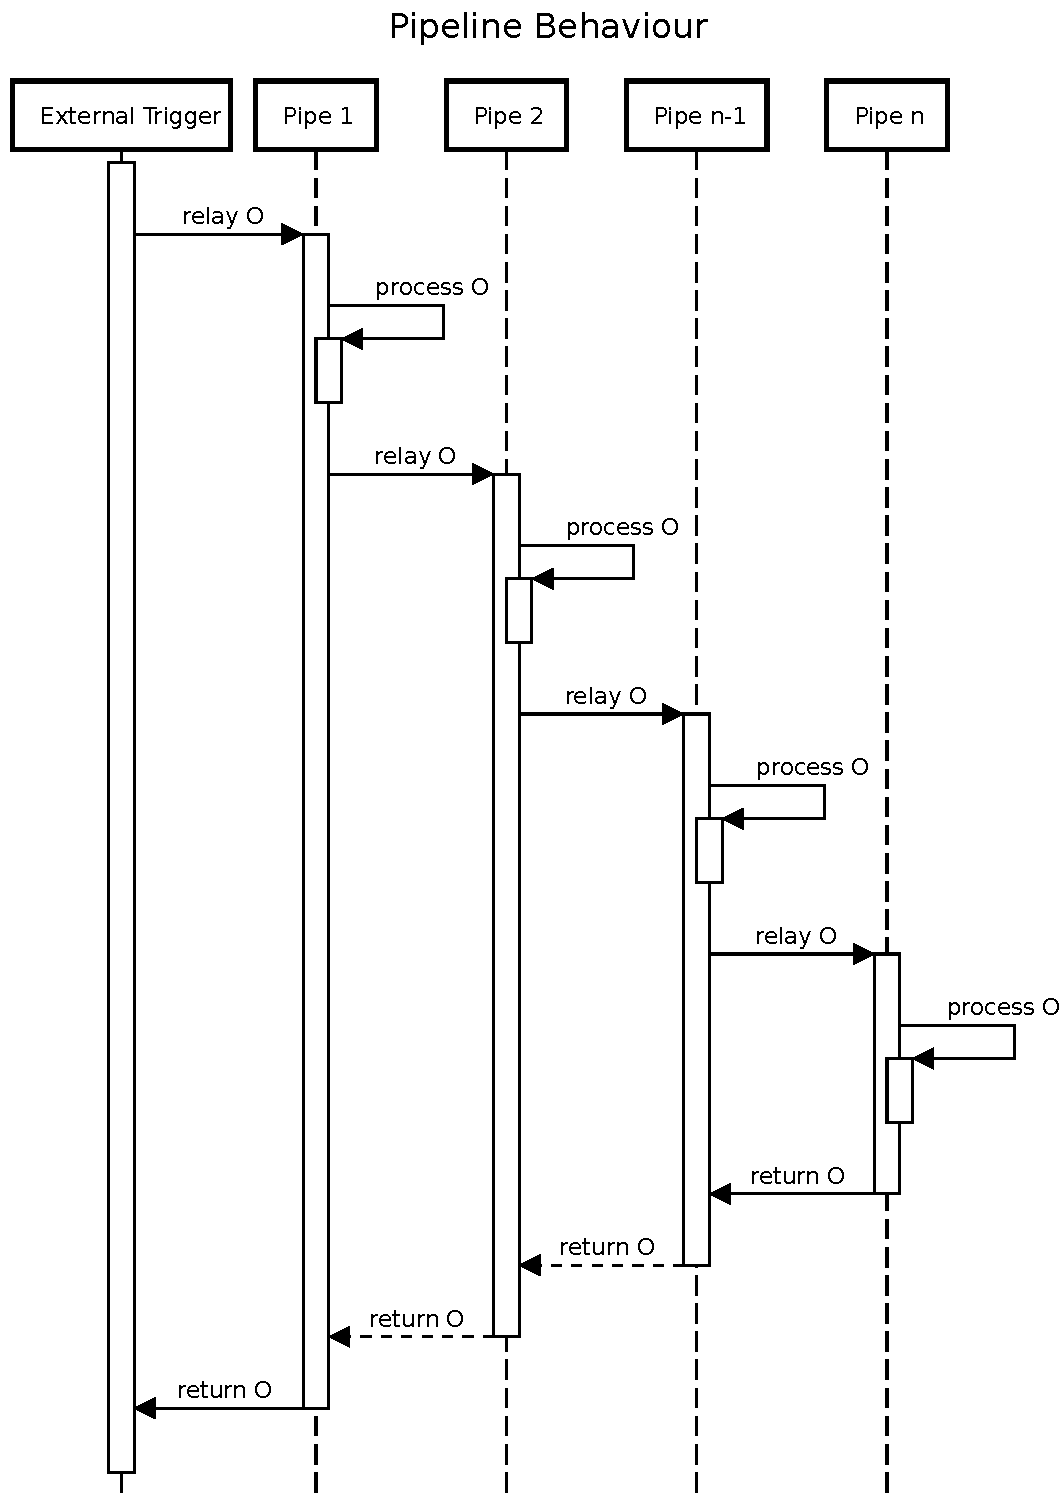
\includegraphics[width=12cm]{img/ch04/pipeline-behaviour.pdf}
    \captionof{figure}{?} % TODO
    \label{fig:dp-pipes-filters}
\end{figure}
\subsection{Abstract Factory Pattern}
%CITE: 1997 - Book - Design Patterns
\subsection{Publish-Subscribe/Observer Pattern}
%CITE: 1997 - Book - Design Patterns

\section{Computer Communication}
\label{sec:computer-networks}
\emph{TBD: OSI-Modell} %TODO
%CITE: ISO/IEC 1994
%TBD: Proxy?

\section{(Industrial) Internet of Things}
\label{sec:internet-of-things}
\subsection{Fields of Use}
%TBD: KRITIS
%CITE: 2013 - Book - BSI
%Smart Home?
\subsection{Application Architectures}
\emph{TBD: Cloud + Device}
\subsection{Common Protocols}
\label{sec:iot-common-protocols}
Building up on pre-existing network infrastructure and in order to meet requirements specific to individual fields of use and use-case scenarios, the landscape of \ac{IoT} attends with a great variety of \emph{communication protocols} (further used to refer to both transport and application protocols). This section will provide a brief overview of the working principles, use cases and history of some protocols commonly used in \ac{IoT} and \ac{IIoT} applications today.
\paragraph{\ac{HTTP}} \emph{TBD} %TODO
\ac{HTTPS}
%CITE: 1.0 https://datatracker.ietf.org/doc/html/rfc1945
%CITE: 2019 - Book - SmartInnovationsInCommunicatio - p174
\paragraph{\ac{WS}} \emph{TBD}

%CITE: https://datatracker.ietf.org/doc/html/rfc6455
%CITE: PMCE https://tools.ietf.org/html/rfc7692
\paragraph{\ac{MQTT}}
\cite{gupta_banks_2015}

\paragraph{Industrial} Modbus \ac{TCP}, Profibus/Profinet, \ac{OPC U/A}

\section{Information Security}
\label{sec:information-security}
\subsection{The CIA Triad}

\subsection{Penetration Testing}

\subsection{Man-In-The-Middle Attacks}
\ac{MITM}
%Cite: A Survey of Man In The Middle Attacks

\subsection{Tools}
There are many tools used in information security. They vary greatly in their features, field of use and maturity. The following paragraphs describe tools relevant to this thesis and the fields of use it touches.

\paragraph{Wireshark} First released in 1998, \emph{Wireshark} is a cross-platform and open-source tool used for network analysis, including \emph{network sniffing} \cite{wireshark}. It is written mainly in C, consists of more than 3,600,000 lines of C code\footnote{This number was returned by the \emph{cloc} utility run on commit \emph{c73ab16b} from 23rd May 2021 of Wireshark's GitLab source-code repository \cite{wiresharkgit}.} and features a \ac{GUI}. Although it is described as a network protocol analyser, it also supports sniffing of \ac{USB} packets. It implements a wide array of \emph{dissectors} for various protocols and allows detailed examination of network packets (as shown in figure \ref{fig:wireshark}).

\begin{figure}[h]
    \centering
    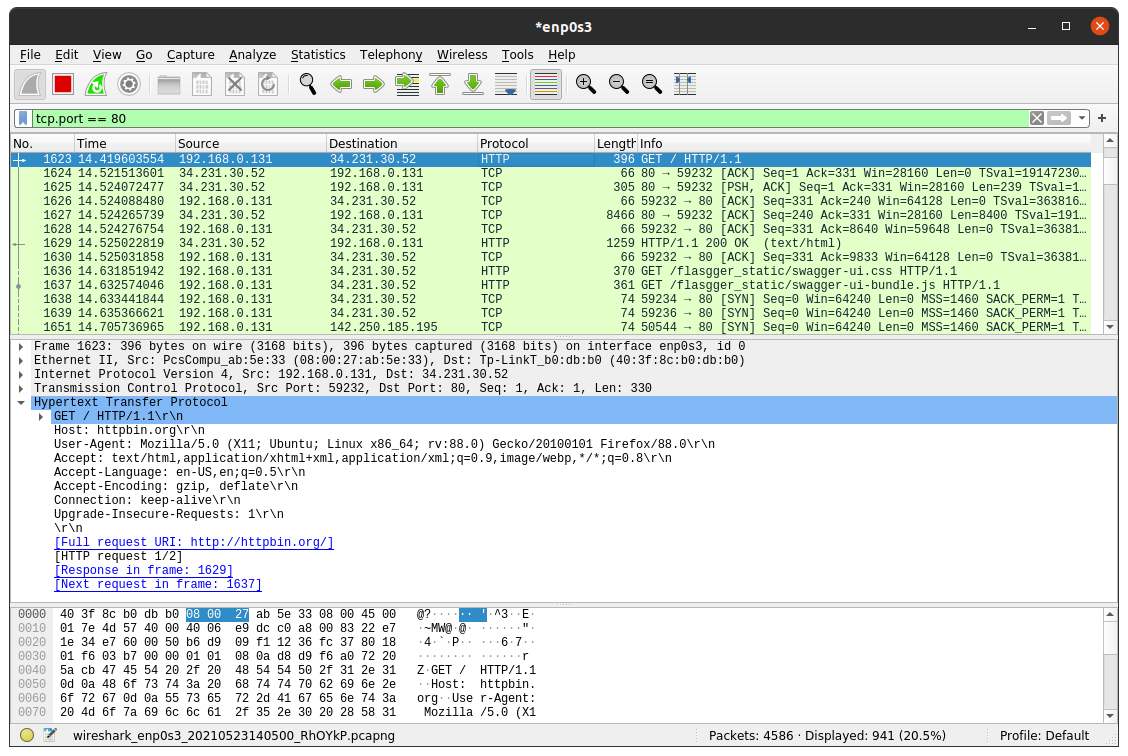
\includegraphics[width=14cm]{img/ch03/wireshark.png}
    \captionof{figure}{Screenshot of Wireshark being executed and dissecting a \ac{HTTP} $GET$ request to the site \enquote{httpbin.org}. The display-filter \enquote{tcp.port == 80} shows only packets sent to or from port 80 (e.g. \ac{HTTP} communication).}
    \label{fig:wireshark}
\end{figure}

\subsubsection{Specific \acp{MITM}}
The following tools are \acp{MITM} that support specific protocols only:
%Specific mitms:
\paragraph{Burp Suite} Developed and distributed by \enquote{PortSwigger} as a commercial product, \emph{Burp Suite} is a tool specialized for web-application testing \cite{burpsuite}. It can be used as a \ac{MITM} for \ac{HTTP} communication by configuring the operating system or browser to use its internal \ac{HTTP} server as a proxy. While it implements basic support for \ac{WS}, it is mainly used for \ac{HTTP} (and nowadays \ac{HTTPS}) and lacks support for other protocols. Aside from its internal proxy server, it also provides specialized features such as the \enquote{Repeater} which is used to send forged \ac{HTTP} requests. The freely available \enquote{Community Edition} (shown in figure \ref{fig:burpsuite}) allows use of most of the tool's features.

\begin{figure}[h]
    \centering
    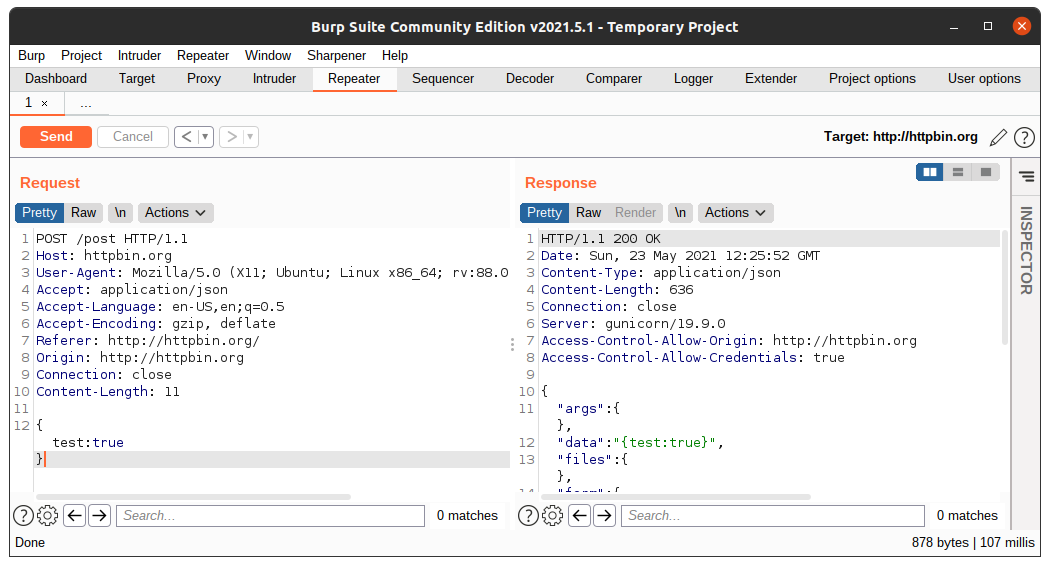
\includegraphics[width=14cm]{img/ch03/burpsuite.png}
    \captionof{figure}{Screenshot of Burp Suite being used to send forged \ac{HTTP} requests to the site \enquote{httpbin.org}.}
    \label{fig:burpsuite}
\end{figure}
\paragraph{mitmproxy} %focused on HTTP/S + WS but supports extension, largely undocumented source
\paragraph{mProxy}
\paragraph{IOXY}
%Generic
\subsubsection{Generic \acp{MITM}}
The following tools are generic \acp{MITM} that support a wide range of network protocols:
\paragraph{ettercap} While \emph{ettercap} was initially developed as a network sniffer for switched \ac{LAN}, it was gradually extended to implement a set of \ac{MITM} attacks such as \ac{ARP} spoofing and \emph{packet filtering} which allowed modifying intercepted communication \cite{ettercap}. Penetration testers can write custom filters in a scripting language to implement their own packet filtering logic. It is written in C and implements network protocols of layers 1 to 4 of the \ac{OSI} model. Thus, it does not implement application protocols.
\paragraph{bettercap} Similar to ettercap, \emph{bettercap} implements network sniffing and other features used for network analysis and discovery. However, contrary to ettercap, it aims to support a wider range of transport technologies and is described as \enquote{\emph{the Swiss Army knife for WiFi, Bluetooth Low Energy, wireless HID hijacking and IPv4 and IPv6 network reconnaissance and MITM attacks}} \cite{bettercap}. It is written in Go and features a web-interface for configuration, control and monitoring.
\paragraph{Scapy}
\paragraph{MITMf} %Built on scapy, implements some attacks and servers, not maintained anymore, superseded by bettercap 
%4. Problem space (Prototype, test setups, existing software)
\chapter{Understanding the Problem Space}
\label{chap:understanding-the-problem-space}
In order to provide a satisfying solution to the problem at hand, the problem itself and the environment it occurs in must be researched. This chapter aims to explore and examine the problem space, resulting in a set of artefacts (namely a domain model and a set of requirements) that aid in understanding the context and designing an appropriate solution. First, a prototypical network proxy is designed and implemented in section \ref{sec:prototypical-implementation} to get an understanding of the problems and challenges involved in designing, implementing and using such software. Based on these experiences, interviews with experts in penetration testing are conducted and evaluated in section \ref{sec:interviews} to get a proper understanding of their everyday work and resulting problems. Lastly, existing software that aims to intercept communication for various scenarios and technologies is examined in section \ref{sec:analysis-existing-software}, compared to each other and their usefulness for the problem-specific scenarios is assessed.

\section{Prototypical Implementation}
\label{sec:prototypical-implementation}
The prototype was designed to be used in three different scenarios, each taking place in a different context. The goal of this section was to implement a prototype that could be used as a proxy to intercept communication between an \ac{IoT} device and its cloud service as shown in figure \ref{fig:network-communication-diagrams}. It was developed incrementally so individual components could be derived from requirements, designed, implemented and evaluated in fixed sprints.

\begin{figure}%
    \centering
    \subfloat[\centering Regular communication between an \ac{IoT} device and a cloud service.]{{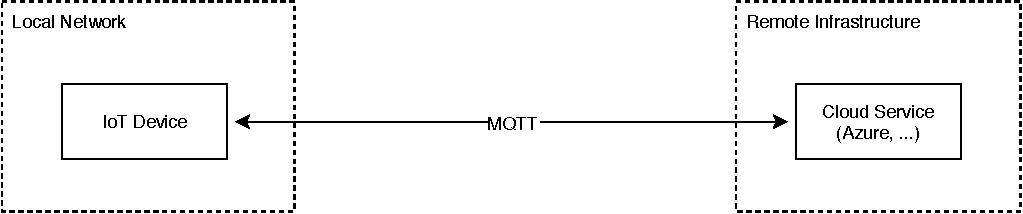
\includegraphics[width=10cm]{img/ch04/Setup - 1 Regular.pdf} }}%
    \qquad
    \subfloat[\centering Communication intercepted by a \ac{MITM} proxy.]{{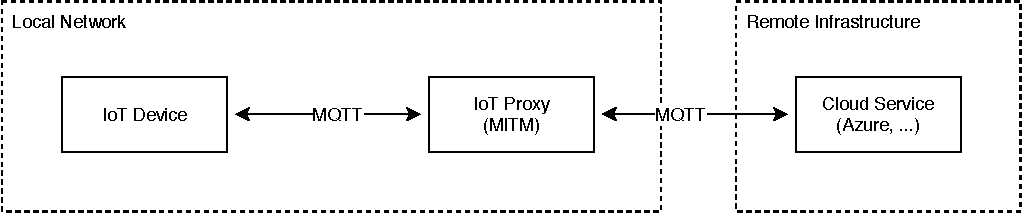
\includegraphics[width=10cm]{img/ch04/Setup - 2 Pentesting.pdf} }}%
    \caption{Installing a \ac{MITM} proxy to intercept network communication for penetration testing.}%
    \label{fig:network-communication-diagrams}%
\end{figure}

\subsection{Example Scenarios}
\label{sec:example-scenarios}
The following scenarios describe hypothetical configurations of \ac{IoT}/\ac{IIoT} devices that should be tested with the prototype and vary in both technical and logical complexity as well as in closeness to reality:

\paragraph{Scenario \#1: Legacy \ac{ICS} Application}
In this \ac{IIoT} scenario, a \ac{HMI} (\emph{Siemens KTP400 Basic}) sends commands to and receives data from a \ac{PLC} (\emph{Siemens S7-1200}) using Modbus \ac{TCP}. The \ac{PLC} continually counts up a value up to 100 and begins anew at zero while the \ac{HMI} displays the current value and provides a button that, upon being pressed by a user, resets the current value to zero. \\
In this scenario, attackers could perform a variety of attacks on the system by intercepting and manipulating network traffic, for example:
\begin{itemize}
    \item By dropping messages sent from the \ac{PLC} to the \ac{HMI}, the application may appear unresponsive as new data is not displayed on the \ac{HMI}. In production environments, this could lead to dangerous situations as sensor readings that indicate harmful environmental conditions would not be presented to supervising personnel.
    \item When dropping messages sent from the \ac{HMI} to the \ac{PLC}, control commands can be suppressed. This attack can result in catastrophic situations when emergency shutdowns issued by supervising personnel are not registered by the affected machines.
\end{itemize}
This scenario is of an academic nature and does not depict a realistic \ac{ICS} process, but focusses on the use of a legacy transport protocol. Due to the rather simple nature of the Modbus \ac{TCP} protocol, intercepting and manipulating communication is expected to be trivial. %TODO: Add diagram?
%https://support.industry.siemens.com/tf//WW/en/posts/s7-1500-communication-and-modbus-tcp-on-hmi/144092?page=0&pageSize=10
%https://support.industry.siemens.com/cs/pd/379924?pdti=td&dl=en&lc=en-DK

\paragraph{Scenario \#2: \ac{IoT} Cloud Application} This \ac{IoT} smart home scenario utilizes two local \ac{IoT} devices that are integrated into a cloud environment such as the \ac{AWS} \ac{IoT} platform: a thermometer and an \ac{A/C} unit. Both devices connect to the cloud platform, authorize themselves at a \ac{REST} interface via \ac{HTTP} and upgrade their \ac{HTTP}-connection to \ac{WS} streams upon successful authorization. They eventually communicate to a remote \ac{MQTT} broker by tunnelling \ac{MQTT} packets over the \ac{WS} stream. At this stage, the thermometer publishes temperature readings to an \ac{MQTT} topic while the \ac{A/C} unit subscribes to the same topic and adjusts its operation depending on the incoming temperature readings. \\
This distributed communication setup introduces a set of possible attacks that could be performed when attackers \emph{impersonated} client-devices or the remote server:
\begin{itemize}
    \item Impersonating the thermometer, attackers could send incorrect temperature data and effectively control the \ac{A/C} unit. When sending low temperature readings while the environment temperature is high, the \ac{A/C} unit would stop running. Conversely, when high temperature readings are sent while the environment temperature is low, the \ac{A/C} unit would run, and thus further cool down the environment.
    \item Attackers that impersonate the remote server could drop or manipulate incoming publish packets, thus altering whether and/or what information is relayed other connected devices. For example, temperature readings that indicate a high environment temperature that would lead to the \ac{A/C} unit to be powered up could be rewritten in such a way that the transmitted temperature value is considered to indicate a low environment temperature, thus preventing the \ac{A/C} unit from running automatically.
\end{itemize}

\begin{figure}[ht]
    \centering
    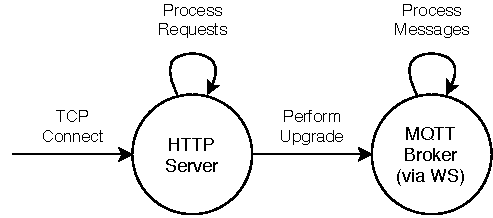
\includegraphics[width=6cm]{img/ch04/Statemachine 2.pdf}
    \captionof{figure}{State machine of \ac{AWS} \ac{IoT} communication}
    \label{fig:aws-statemachine}
\end{figure}
This scenario makes use of three communication protocols, uses these protocols dependent on the state of authentication and even tunnels one protocol through another one. Therefore the proxy application has to implement a state-machine (as seen in figure \ref{fig:aws-statemachine}) and testing communication in this scenario is expected to be more complex than the first one. Also, since this scenario makes use of the \ac{AWS} \ac{IoT} infrastructure, special care must be taken to ensure that authentication is properly relayed to the cloud servers.

% Reference: https://aws.amazon.com/blogs/aws/aws-iot-cloud-services-for-connected-devices/

\paragraph{Scenario \#3: Water Treatment Plant} Similar to scenario \#2, this scenario makes use of \ac{MQTT} for transporting messages. However, the scenario takes place in an \ac{ICS} context of critical infrastructure.

\begin{figure}[hb]
    \centering
    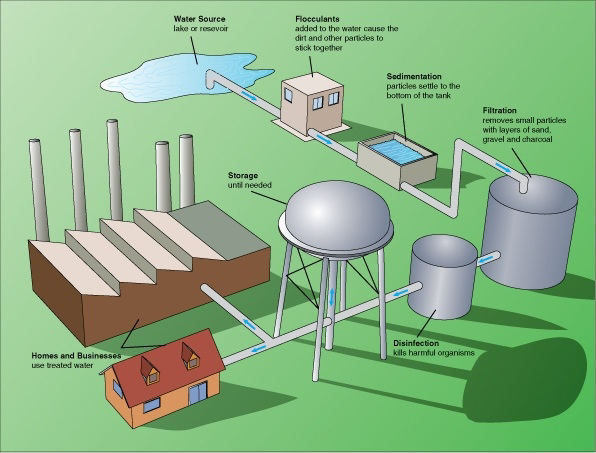
\includegraphics[width=12cm]{img/ch04/watertreatmentplant.png}
    \caption[Illustration of a typical drinking water treatment process. (by the CK-12 Foundation)]{Illustration of a typical drinking water treatment process. (by the CK-12 Foundation)\protect\footnotemark}
    \label{fig:water-treatment}
\end{figure}
\footnotetext{https://en.wikipedia.org/wiki/File:Illustration\_of\_a\_typical\_drinking\_water\_treatment\_process.png}

As shown in figure \ref{fig:water-treatment}, there are multiple steps involved in treating water for drinking. The scenario represents these steps as separate stations (\enquote{source}, \enquote{flocculants}, \enquote{sedimentation}, \enquote{filtration} and \enquote{storage}) that act as \ac{MQTT} clients. Each station receives water into an input tank, processes water from its input tank in a specified rate and flushes processed water into an output tank. Similar to how threads can suffer from starvation in a multithreading environment, these stations can either \enquote{run dry} when their input tank is empty or overflow when either tank is filled beyond their capacity. In this scenario, stations will only process water from their input tanks if their output tank provides sufficient available capacity.\\
Similar to scenario \#2, attackers could perform a series of attacks in this scenario:
\begin{itemize}
    \item Without intercepting any communication, attackers could cyclically overwrite water levels of either input and output tanks to stop stations and bring processing to a halt. For example, when attackers overwrite the \enquote{storage} station's input tank level to indicate exhausted capacities, the \enquote{disinfection} station would fill its output tank and eventually stop processing water. This would cause the \enquote{disinfection} station's input tank to fill up and lead to the \enquote{filtration} station's output tank to fill up. Ultimately, the water treatment plant would halt.
    \item When any station publishes data about its tanks' levels indicating full or empty capacities, attackers could intercept those messages and change them to either indicate the opposite (change tank levels indicating \emph{full} capacities to levels indicating \emph{empty} capacity) or some arbitrary level information. This could lead to either pumping water from empty tanks, potentially damaging the pumps, or to overfilling tanks, leading to leaking excess water and potentially damaging further equipment.
\end{itemize}
This scenario greatly simplifies drinking water treatment by reducing the process to the producer-consumer problem known from multithreading. A more realistic representation of drinking water treatment plants would take further details, such as chemicals used in disinfection, into account.\\
This scenario involves only \ac{MQTT} as a transport protocol but requires six \ac{MQTT} clients to run simultaneously.

\paragraph{Derived Use-Cases} A number of simple %High-level, abstrahiert?
use-cases (shown in \ref{fig:use-cases-scenarios}) can be derived from these scenarios. The actors are the \enquote{Attacker} that intend to interact with the system in a malicious way, the \enquote{Server} and \enquote{Client} that use the system for transportation of messages. The following use-cases are found in the aforementioned scenarios:

\paragraph{Send/Receive Messages:} Used by \enquote{Server} and \enquote{Client} to

\begin{figure}
    \centering
    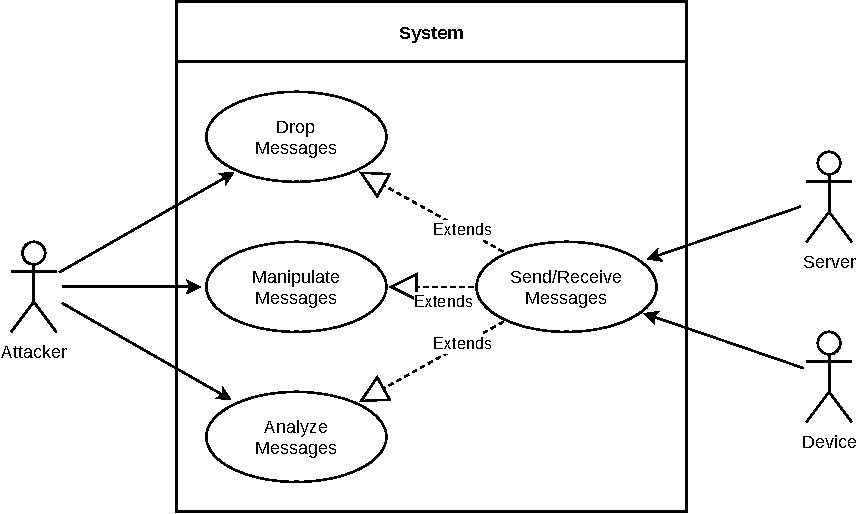
\includegraphics[width=14cm]{img/ch04/UseCases_Scenarios.pdf}
    \captionof{figure}{The variation of the \emph{\enquote{pipes and filters}}/\emph{\enquote{pipeline}} design pattern used in the prototype.}
    \label{fig:use-cases-scenarios}
\end{figure}

\subsection{Requirements}
To be able to operate in all of the aforementioned scenarios, the prototype had to implement a set of functional requirements:
\begin{itemize}
    \item [\textbf{F1}] \textbf{Protocols:} The software must implement parsing/crafting messages/packets of the following communication protocols: \ac{HTTP}, \ac{WS}, \ac{MQTT} and Modbus \ac{TCP}. \\
          \textbf{Fit criterion:} The software must implement and support the \ac{HTTP}, \ac{WS} and \ac{MQTT} protocols so messages of those protocols can be further processed by the software.
    \item [\textbf{F2}] \textbf{Network Stacks:} The software must be able to parse protocols that are tunnelled through other protocols (\enquote{\emph{stacked}}). It must provide an interface to the user where they can specify which communication protocols are used and whether and how they are stacked (further referred to as \emph{network stack}).\\
          \textbf{Fit criterion:} The software processes a configuration file that lets users specify which protocols to be used and whether/how they are stacked.
    \item [\textbf{F3}] \textbf{State-Machines:} The software must be able to switch network stacks and scripts for processing dependent on configurable \emph{states} and \emph{transitions} between them. It must provide an interface for the user to specify when to switch to using another network stack, represented using \acp{FSM} and rule sets for transmission between states.\\
          \textbf{Fit criterion:} The software processes a configuration file that lets users specify when to switch between network stacks.
    \item [\textbf{F4}] \textbf{Integration:} The software shall provide interfaces for integration of third-party software.\\
          \textbf{Fit criterion:} The software implements interfaces that allow sending packets to other applications such as \enquote{Burp Suite}.
    \item [\textbf{F5}] \textbf{Scripting:} The software shall provide scripting capabilities for automated manipulation of messages/packets.\\
          \textbf{Fit criterion:} Users can define script-snippets to be executed on messages/packets.
\end{itemize}

The following non-functional requirements were defined:

\begin{itemize}
    \item [\textbf{N1}] \textbf{Extensibility:} To allow for future implementation of further communication protocols the software shall be implemented in a modular fashion.
    \item [\textbf{N2}] \textbf{Platform Compatibility:} In order to support a broad spectrum of target platforms, the software shall be implemented platform-independently.
    \item [\textbf{N3}] \textbf{Reusability:} The software shall be reusable so it can be used in future tests that may feature new configurations of network stacks.
    \item [\textbf{N4}] \textbf{Open Source:} The software shall be available as open source software so programmers and members of the IT community may contribute to improving it.
\end{itemize}

Due to this implementation serving as a prototype and being of an academic nature, no specific constraints were defined. It was to be developed strictly ignoring aspects of usability and stability as it should not be used in production environments but in laboratories exclusively.

\subsection{Design}
The prototype was designed to be fit for use in the second scenario as, regarding network communication, it was more complex than the other ones. Specifically, the second scenario demanded the implementation of a network stack and a state machine to switch between states.
Parsing protocols that were tunnelled through other protocols appeared to be a potentially challenging requirement. In order to tackle it, a variation of the \emph{\enquote{pipeline}} (sometimes referred to \emph{\enquote{pipes and filters}}) design pattern was used (as shown in figure \ref{fig:design-pipes-and-filters}). It was designed to be used as follows:\par
\enquote{Messages} originate from a listener, for example messages with raw byte payloads are received from a \ac{TCP} socket. These messages are sent to an initial \enquote{pipe} to be processed \emph{down}.
Pipes are bi-directional routers that perform the following actions on messages:
\begin{enumerate}
    \item Use optional \enquote{encoders} to disassemble/de-serialize messages when processing them \emph{down} the pipeline and re-assemble/serialize them when they process messages \emph{up} the pipeline.
    \item Use optional \enquote{filters} to perform operations on messages such as replacing header values or manipulating payloads.
    \item Forward messages to the next pipe in its pipeline when processing messages down or to the previous pipe when processing messages back up.
\end{enumerate}
There are extensions to basic pipes such as:
\begin{itemize}
    \item \enquote{EndPipes} are appended to the end of a pipeline and reverse the message processing direction so messages that were processed down are sent back up the pipeline to be processed up.
    \item \enquote{ProcessingPipes} mandate encoders and filters to be used. These pipes are used to indicate that messages are not not only routed but also processed and encoded or decoded.
    \item \enquote{IntegrationPipes} allow integration of other software into the pipeline. For example, penetration testing software such as Burp Suite could be integrated.
\end{itemize}

\emph{TBD:}
\begin{itemize}
    \item \emph{Designed during sprints so only pipes are designed, state-machine only rough concept (States, Transitions, Rules)!}
    \item \emph{Show diagrams of messages?}
    \item \emph{Explain Figure \ref{fig:app-diag-pipesfilters-1} and \ref{fig:app-diag-pipesfilters-2}}
\end{itemize}


\begin{figure}
    \centering
    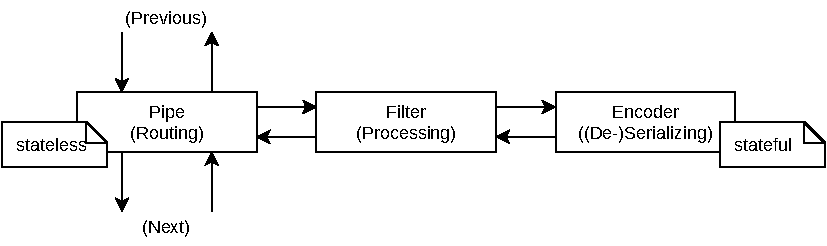
\includegraphics[width=14cm]{img/ch04/Architecture - Pipes and Filters3.pdf}
    \captionof{figure}{The variation of the \emph{\enquote{pipes and filters}}/\emph{\enquote{pipeline}} design pattern used in the prototype.}
    \label{fig:design-pipes-and-filters}
\end{figure}

\subsection{Testing}
\label{sec:prototype-testing}
To test the prototype, a simple testbed was designed and implemented to realize scenario \#3 (discussed in section \ref{sec:example-scenarios}). It consisted of two Debian 10 machines that acted as a \ac{MQTT} broker and clients and a Kali Linux machine that ran the prototype and provided tools such as Wireshark that could be used for debugging and monitoring network traffic. All machines were connected to a single network (shown in figure \ref{fig:testbed}) and were assigned static \ac{IP} addresses. While this setup allowed for more sophisticated \ac{MITM} mechanisms such as \ac{ARP} spoofing, the decision was made to directly connect the \ac{MQTT} clients to the \emph{kali} machine to reduce complexity and accelerate and simplify testing. Separate machines were used for the \ac{MQTT} broker and clients so that actual \ac{MITM} attacks could be performed if the need to arose. Also, running the broker on a separate machine simplified debugging as network traffic could be attributed to broker or clients easier by examining the packets' source and destination \acp{IP}.\par

\begin{figure}[h]
    \centering
    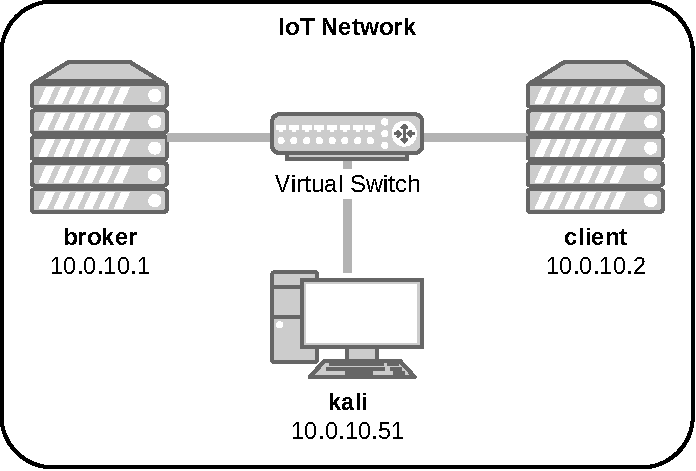
\includegraphics[width=8cm]{img/ch04/Testbed2.pdf}
    \captionof{figure}{A network diagram of the testbed that was used for testing the prototype.}
    \label{fig:testbed-network}
\end{figure}
The \ac{MQTT} broker software used on the \emph{broker} machine was Eclipse Mosquitto\footnote{https://mosquitto.org/} $1.5.7$ and had the \ac{WS} transport enabled to allow for clients to connect via \ac{WS}. The \ac{MQTT} clients running on the \emph{client} machine were implemented in Python using the Eclipse Paho library for Python (paho-mqtt\footnote{https://pypi.org/project/paho-mqtt/}).\par %TODO: Describe publish and processing pattern, ref mqtt graph below
\begin{figure}[h]
    \centering
    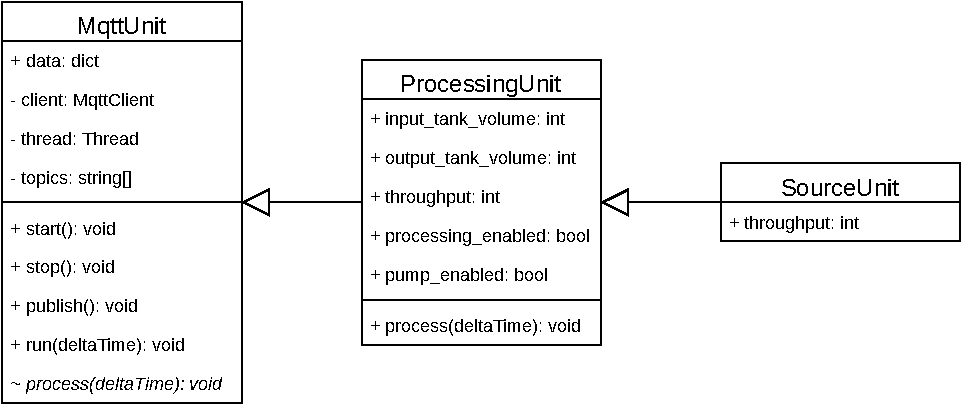
\includegraphics[width=14cm]{img/ch04/Testbed-Unit.pdf}
    \captionof{figure}{The \enquote{ProcessingUnit} data-structures represent individual stations of the simplified water treatment plant.} %TODO: Describe
    \label{fig:testbed-unit}
\end{figure}
The water treatment scenario required water treatment stations to be simulated individually as separate \ac{MQTT}, which was done by representing them as \enquote{ProcessingUnits} in the Python implementation of the testbed. As can be seen in figure \ref{fig:testbed-unit}, ProcessingUnits held individual \emph{MqttClient} instances running in separate threads, were subscribed to the topics of relevant other units such as their direct predecessors and successors and were capable of publishing their current state. Their \emph{process} method would be called cyclically and allow for units to calculate their intake, throughput and output.

\begin{figure}[h]
    \centering
    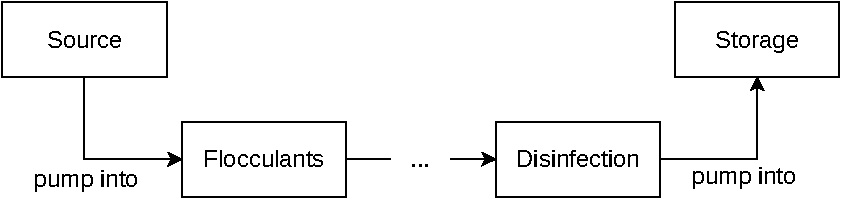
\includegraphics[width=12cm]{img/ch04/Testbed-Chain.pdf}
    \captionof{figure}{Chaining of the water treatment units, originating from a water source and eventually leading to a storage at the end of the processing pipeline.} %TODO: Describe
    \label{fig:testbed-chain}
\end{figure}
These units were then \enquote{chained} up (shown in figure \ref{fig:testbed-chain}) in the order in which they were presented in the scenario by specifying their direct predecessor and successor units: potentially contaminated water would be pumped out of the \emph{source}, processed by a series of stations and eventually flushed into the \emph{storage}. The \emph{source} was an instance of the \enquote{SourceUnit} that featured a throughput calculated by a sine-wave function that used the elapsed time since program startup as input parameter. Also, in order to keep the program running infinitely without either the \emph{source} \enquote{running dry} due to its input tank emptying or the \emph{storage} overfilling, the \emph{storage's} output was programmed to feed back into the \emph{source's} input tank (as can be seen in figure \ref{fig:mqtt-data}). While this was not a realistic approach, it kept the program's design simple and allowed for continuous testing and did not impact the \ac{MQTT} communication.

\begin{figure}[h]
    \centering
    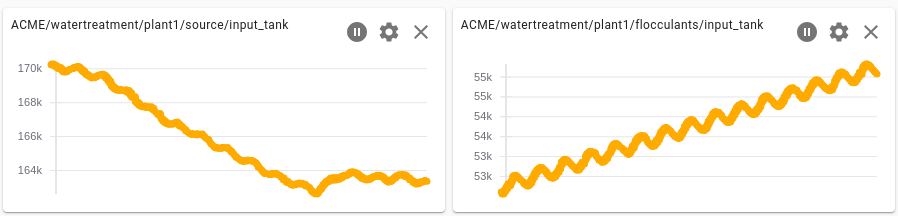
\includegraphics[width=14cm]{img/ch04/watertreatment-mqtt-short.png}
    \captionof{figure}{Screenshot of the application \enquote{MQTT Explorer} that was used to inspect and visualize the state of the water treatment plant. The left graph shows how the \emph{source's} input tank steadily emptied until it was filled by the \emph{storage's} output tank. The right graph shows how the \emph{flocculant} unit's input tank slowly filled up.} %TODO: Describe
    \label{fig:mqtt-data}
\end{figure}

\subsection{Implementation}
\emph{TBD:}  %TODO: Write out
\begin{itemize}
    \item \emph{technology: typescript}
    \item \emph{sprints: two sprints, started with communication (http + ws + mqtt)}
    \item \emph{failed: high-level API, callback-hell (debugging/tracing), missing typescript typings, very tight coupling}
\end{itemize}

\subsection{Insights Gained}
The following insights were gained through the prototypical implementation. Some resulted in questions relevant for the expert interviews that were to be held:
\begin{itemize}
    \item Due to the \ac{MTU}, large messages are broken into chunks that are transferred sequentially. This requires the proxy to work on streams of incoming data and reassemble messages from said chunks. % TODO: Also, stateful + buffers per connection
    \item Support of multiple clients is non-trivial as communication between clients and servers is not necessarily connection-oriented (e.g. \ac{HTTP}).\\
          \emph{Q: Do penetration testers need to test multiple devices at the same time?}
    \item Increasing the size of the payload of a messages can result in the payload being split upon multiple messages (e.g. \ac{WS}).\\
          \emph{Q: Do penetration testers require exact control over the implementation of protocols?}
    \item Manipulating messages, on the fly via scripting or by hand using third-party integrations (e.g. to \emph{Burp Suite}), can introduce latency to the communication. \emph{Q: Are there strict timing requirements during penetration tests?}
    \item Many libraries offer high-level functions to the programmer while avoiding exposure of low-level functionalities like crafting or parsing messages.
\end{itemize}


\section{Interviewing Experts for Insights}
\label{sec:interviews}
Interviews may be an efficient way to get an expert’s opinion on something they are proficient in. Thus, expert interviews were conducted to let security researchers give insight into their everyday work and the challenges they face when working with \ac{IoT} and \ac{IIoT} applications. The information and insights gathered in these interviews were then used to model a persona, various work scenarios and use-cases that as a whole aim to represent their work.

\subsection{Interview Guideline}
An interview guideline (shown in \emph{TBD}) %TODO: Reference appended interviews + guideline
was created to keep focus on key points during interviews so that interviewees would not stray too far from the relevant points. The guideline also served as a checklist so the interviewer could make sure that all questions and points that should be covered  initially, were in fact covered by the end of the interviews. It was composed of three sections:

\paragraph{1. Experiences with IoT} The answers to these questions would give insights into what kind of applications the security researchers had worked on in the past. Answers to question \emph{1.1.} were of particular interest as they might represent what technologies were being examined by security researchers and may be popular in today’s applications.
\paragraph{2. Processes in Everyday Life} This section aimed to cover questions about the processes and tasks security researchers perform during penetration tests of IoT applications in their everyday life. Ideally, answers to those questions would show the approaches taken and challenges faced during their work, uncovering potential needs and underlying motivation.
\paragraph{3. The Future of IoT} This section had security researchers assess what the future of IoT may be like from their point of view. This required the interviewees to make a critical assessment of the status quo.


\subsection{Conducting Interviews}
Interviews were conducted with six %Patrick, Cédric, Théo, Oliver, Pierre, Jonah
\emph{NVISO} employees that all had worked on security assignments on \ac{IoT} or \ac{IIoT} applications in the past. There is considerable variety in
\begin{itemize}
    \item the experience they had in working on security assignments in general: all interviewees had a strong background in cyber security that reached back multiple years except one who was a working student at \emph{NVISO Labs}.
    \item and the experience they had in working on \ac{IoT}/\ac{IIoT} applications: two interviewees worked on assessing \ac{IoT}/\ac{IIoT} applications only occasionally, one was part of a car manufacturer's automotive security team in the past and three were part of \emph{NVISO Labs} and worked with smart devices on a regular basis.
          % Position? CEO vs. Consultant vs. Working student
          % 
\end{itemize}
The duration of the interviews varied from 45 minutes to two hours depending on the amount and level of detail of information provided by the interviewees and the number of times that the interviewer had to ask further questions.

\emph{TBD:} %TODO: Write out
\begin{itemize}
    \item \emph{Summary of the interviews}
    \item \emph{conclusions drawn}
    \item \emph{personas and user stories -> new requirements!}
\end{itemize}
%TODO: CUT interview files, also make them audio only!

\section{Analysis of Existing Software}
\paragraph{Wireshark} more than 3,400,000 lines of C code\footnote{This number was returned by the \emph{cloc} utility run on commit \emph{3a8111e1c2adcdc0603993c6ed5d20a40f162125} from Aug. 4th 2020 of Wireshark's Github mirror.}\emph{TBD}
\paragraph{MITMf} \emph{TBD}
\paragraph{Ettercap} \emph{TBD}
\paragraph{bettercap} \emph{TBD}
\paragraph{mitmproxy} \emph{TBD}
\paragraph{mProxy} \emph{TBD}
\paragraph{IOXY} \emph{TBD}
\paragraph{scapy} \emph{TBD}

\emph{TBD; planned: paragraph about each program including a general description, uses, capabilities and usefulness} %TODO: Write out
\label{sec:analysis-existing-software}
\begin{table}[h]
    \centering
    \begin{tabular}{r|c|c|c|c|c|c}
        \toprule
        \thead{$Name$} & \thead{$Latest$                                                                                                    \\$Release$} & \thead{$Implemented$\\$in$} & \thead{$Supported$\\$Protocols$} & \thead{$R$} & \thead{$W$} & \thead{$D$}\\
        \midrule
        Wireshark      & 2020-07-01        & C      & Various    & \cellcolor{green!25}F  & \cellcolor{red!25}N    & \cellcolor{red!25}N    \\
        \midrule
        MITMf          & 2015-08-28        & Python & Various    & ?                      & \cellcolor{green!25}F  & \cellcolor{green!25}F  \\ %https://github.com/byt3bl33d3r/MITMf
        \midrule
        Ettercap       & 2019-07-01        & C      & Various    & \cellcolor{green!25}F  & \cellcolor{green!25}F  & \cellcolor{green!25}F  \\
        \midrule
        bettercap      & 2020-03-13        & Go     & Various    & \cellcolor{green!25}F  & \cellcolor{green!25}F  & \cellcolor{green!25}F  \\
        \midrule
        mitmproxy      & 2020-03-13        & Python & HTTP/S, WS & \cellcolor{orange!25}P & \cellcolor{orange!25}P & \cellcolor{orange!25}P \\ %https://github.com/mitmproxy/mitmproxy
        \midrule
        mProxy         & Pre-Releases only & Go     & MQTT       & ?                      & \cellcolor{green!25}F  & -                      \\ %https://github.com/mainflux/mproxy
        \midrule
        IOXY           & Source only       & Go     & MQTT       & \cellcolor{green!25}F  & \cellcolor{green!25}F  & \cellcolor{green!25}F  \\ %https://github.com/mainflux/mproxy
        \bottomrule
    \end{tabular}
    \caption[Comparison of existing software]{Comparison of existing software where $R$, $W$ and $D$ describe read, write and deletion capabilities, respectively. $F$, $N$ and $P$ indicate full, no or partial functionality, respectively.}
    \label{table:comparison-existing-software}
\end{table}
% 4. Konzept (Kontext, Ablauf, Anforderungen [Interviews], Konzept [Architektur])
\chapter{Conceptual Design}
\label{chap:conceptual-design}
%This chapter will detail the process of conceptualizing the design of the modular proxy application based on the results of the preceding chapter. First, the requirements are analysed for their potential design implications in section \ref{sec:req-design-implications}. Afterwards the user interactions and domain entities identified in chapter \ref{chap:understanding-the-problem-space} are examined and broken down into communication flows between actors and systems in section \ref{sec:user-interactions-designing-workflow} and individual software components that complete the design are discussed in section \ref{sec:inferring-software-components}. Lastly, an overview of the complete design concept is given in section \ref{sec:abstract-design-concept}, discussing potential advantages and constraints. %TODO: Rewrite & update

%\section{Inferring Software Components}
%\label{sec:inferring-software-components}
Building on the software design of the first prototype presented in section \ref{sec:prototype-design} and the insights gained in section \ref{sec:prototype-insights}, two design concepts were worked out. The following sections will detail components and principles of both concepts.

\section{Design \#1: Monolithic Proxy Application}
\label{sec:design-1}
This design concept is based on the general ideas presented in section \ref{sec:prototype-design} (e.g. state-machines, network stacks and pipes) and employs a basic architecture shown in figure \ref{fig:component-view-1}.
\begin{figure}[h]
    \centering
    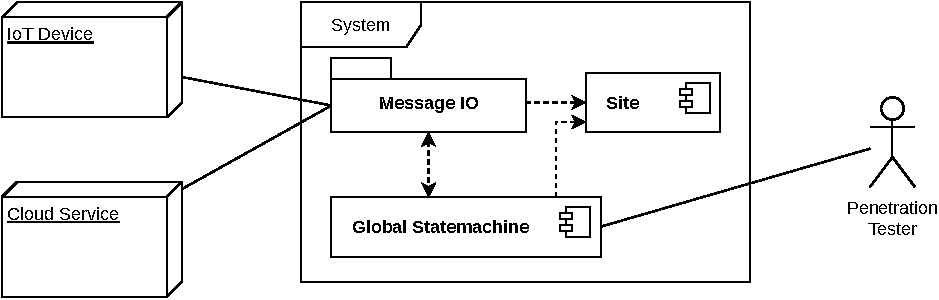
\includegraphics[width=12cm]{img/ch05/component-view-1.pdf}
    \captionof{figure}{High-level component diagram of the proxy application concept}
    \label{fig:component-view-1}
\end{figure}
\subsection{High-level Overview}
As discussed in the previous chapter, the requirement \enquote{F2 Network Stacks} introduces the need for dynamically initialized objects which in this concept is implemented by making use of the abstract factory pattern in the \enquote{Site} component (depicted in figure \ref{fig:site-factory}). This component allows for registering \emph{Factories} that are used to initialize objects. Similar to the implementation in the first prototype, factories initialize objects using metadata supplied from a configuration file.\\
\begin{figure}[H]
    \centering
    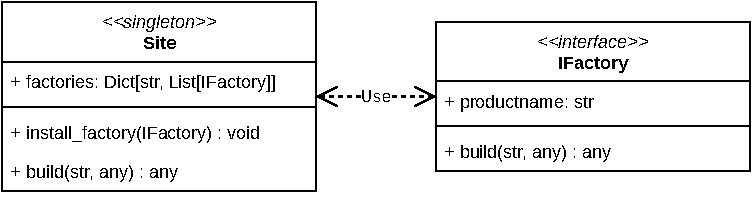
\includegraphics[width=12cm]{img/ch05/site-factory.pdf}
    \captionof{figure}{?} %TODO: Describe
    \label{fig:site-factory}
\end{figure}
Communication with other systems is encapsulated into the \enquote{Message IO}-package shown in figure \ref{fig:component-view-2}. Applications that are tested by penetration testers are connected to sockets provided by the \enquote{Gateway} component and temporarily stored in a message queue to be processed by the network stacks organized by the \enquote{Global Statemachine}. Similar to the \enquote{Server} interface used in the first prototype, gateways provide means of communicating with external systems and receiving and sending messages. They are highly abstract and meant to be used for implementing interfaces for any kind of communication protocols and technologies, such as \ac{IP}-based \ac{TCP} and \ac{UDP} communication but also other protocols such as USB, Bluetooth, ZigBee or KNX.
\begin{figure}[h]
    \centering
    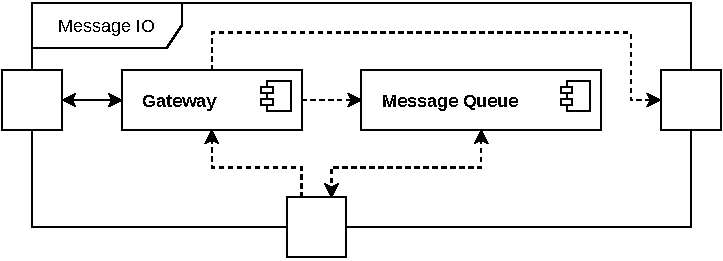
\includegraphics[width=12cm]{img/ch05/component-view-2-messageio.pdf}
    \captionof{figure}{The \enquote{Message IO}-package. The white boxes indicate ports for communication with outside components.}
    \label{fig:component-view-2}
\end{figure}
It should be noted that the static view of the design is rather simple due to its dynamic runtime behaviour: many instances and relationships are only instantiated at runtime and not pre-determined. A schematic representation of the dynamic structure and interweaving of state-machines, network stacks and pipes (in this concept called a \enquote{\emph{pipeline}}) is shown in figure \ref{fig:pipeline}.
\begin{figure}[h]
    \centering
    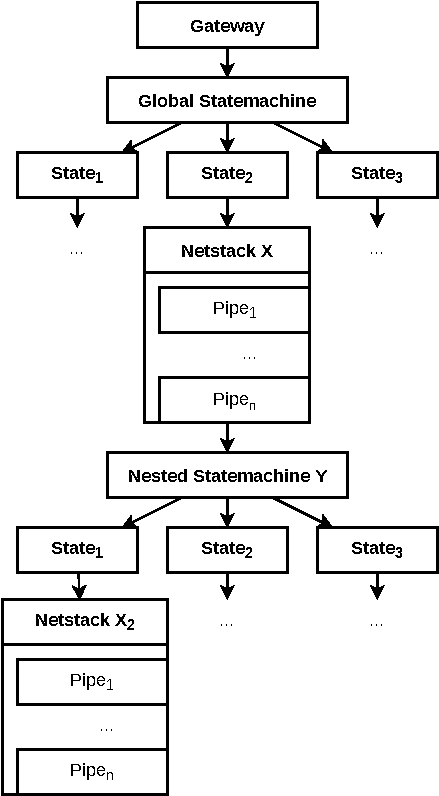
\includegraphics[height=12cm]{img/ch05/pipeline.pdf}
    \captionof{figure}{?} %TODO: Describe
    \label{fig:pipeline}
\end{figure}This figure highlights a series of active state-machines and network stacks which together constitute the active pipeline. \\
\begin{figure}[h!]
    \centering
    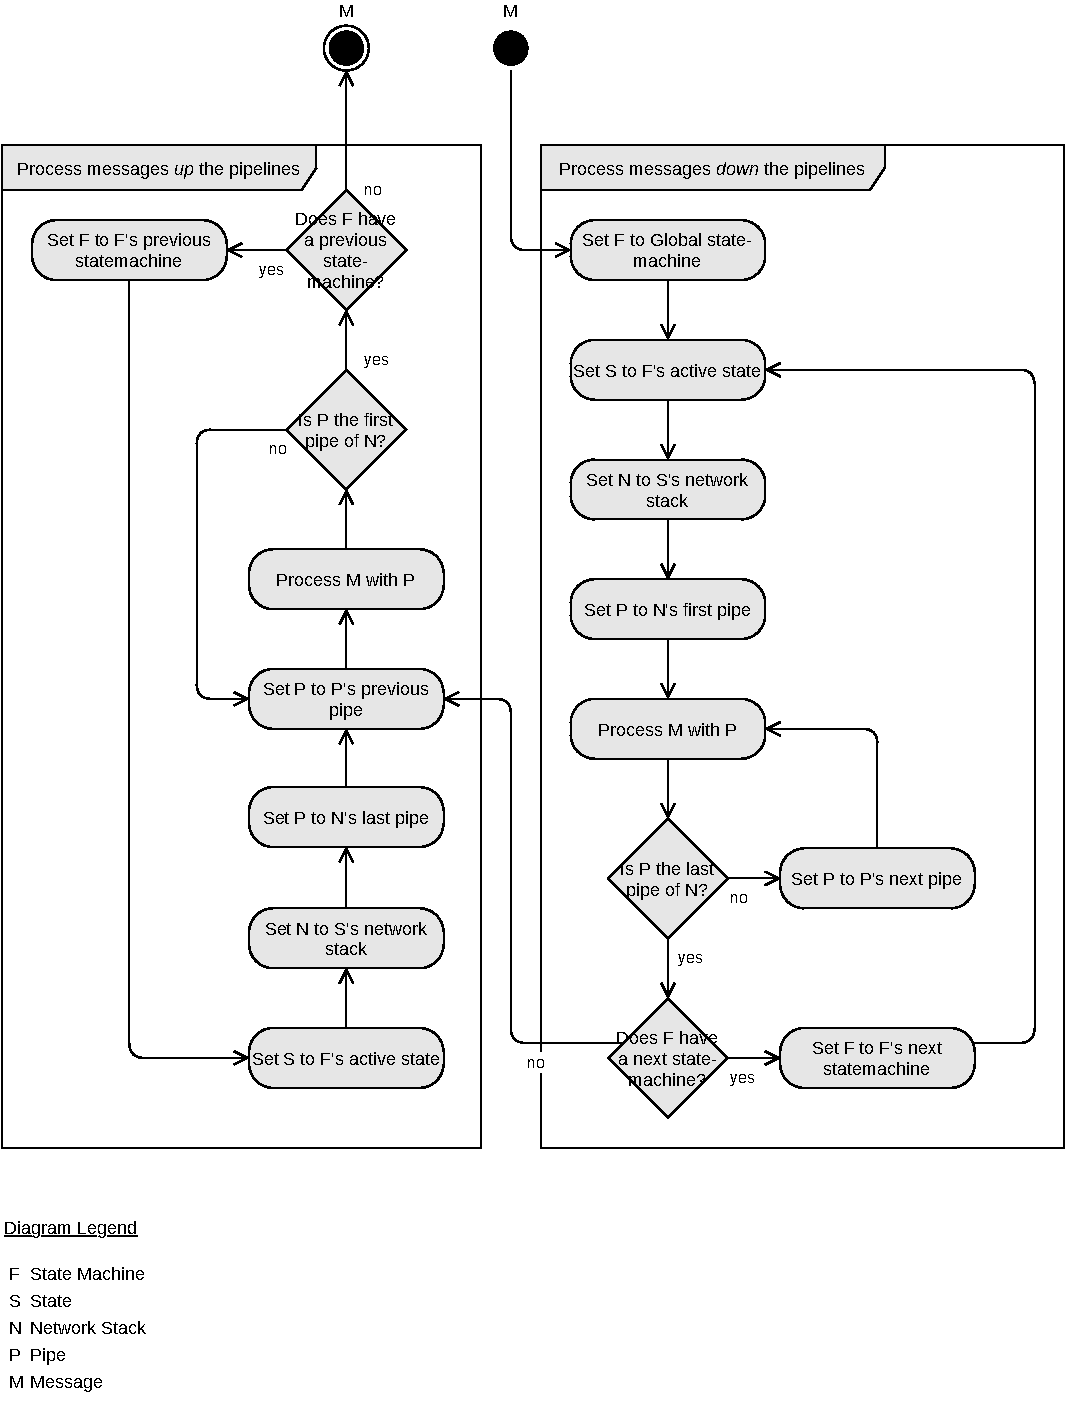
\includegraphics[width=14cm]{img/ch05/activity-nested-fsms.pdf}
    \captionof{figure}{Message processing through an architecture of nested \acp{FSM} and network stacks}
    \label{fig:activity-fsms}
\end{figure}
Figure \ref{fig:activity-fsms} illustrates the recursive nature of this concept processing (dequeued) messages:
\begin{enumerate}
    \item A state-machine $F$ (initialized with the global state-machine instance) relays messages $M$ through its active state $S$'s network stack instance $N$.
    \item In $N$, all of its pipes $P$ process $M$ until the end of $N$ is reached ($P$ does not hold a reference to a succeeding pipe instance). If $F$ holds a reference to a succeeding \ac{FSM}, $F$ is set to this reference and the process continues from step $1$.
    \item If $N$ does not hold a reference to a nested \ac{FSM}, the end of the network stack is reached and the direction of traversing the network stack is reversed.
    \item $P$ is set to $N$'s last pipe instance and $M$ is processed by $P$ until the start of $N$ is reached (i.e. $P$ does not hold a reference to a preceding pipe instance). If $F$ holds a reference to a preceding \ac{FSM} instance, $F$ is set to this reference, $N$ is set to $F$'s network stack reference and the process continues from step $4$.
    \item If $N$ does not hold a reference to a preceding \ac{FSM}, the beginning of the whole pipeline is reached and $F$ is the global state-machine.
\end{enumerate}

\begin{figure}[h]
    \centering
    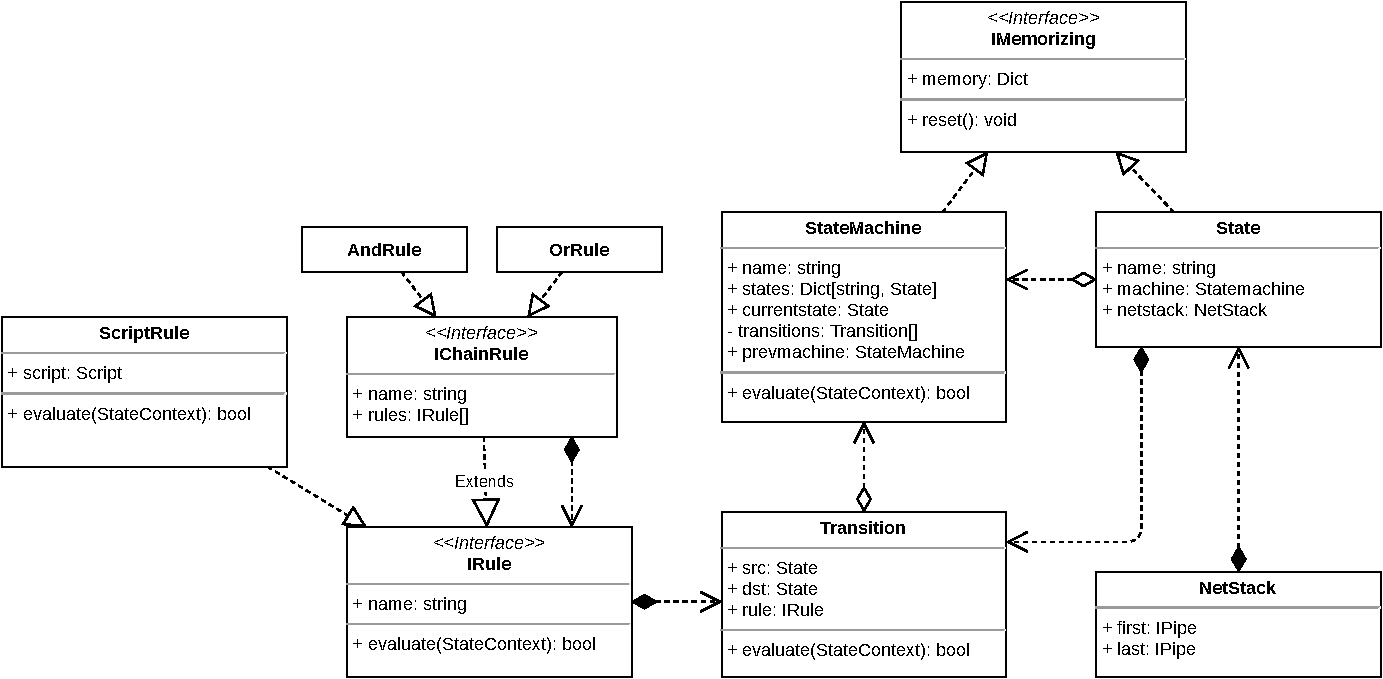
\includegraphics[width=14cm]{img/ch05/classes-1-fsm-rules-netstack.pdf}
    \captionof{figure}{?} %TODO: Describe
    \label{fig:classes-1-fsm-rules-netstack}
\end{figure}
\subsection{State-Machines} The classes related to the state-machine component are shown in figure \ref{fig:classes-1-fsm-rules-netstack}: \emph{StateMachines} hold a set of \emph{States} and \emph{Transitions}. In order to change states, state-machines evaluate a context by checking each of their transitions for whether their conditions for transition are met or not. This context is an aggregation of the \emph{memory} of each state-machine and their active states in the active pipeline. Transitions are defined by a source state, destination state and an \emph{IRule} that evaluates a given context. Rules can be concatenated with logical $AND$ or $OR$ operators and are designed to be scripts that operate on the given context. This allows the creation of nested rules such as the following one:
\begin{align*}
    \mathbf{changeToWS}(c) & = \mathbf{AND}(\mathbf{clientUpgrade}(c), \mathbf{serverUpgrade}(c))
\end{align*}
In this example, a transition with the above rule would evaluate to $true$ and trigger a state transition in a state-machine when the aggregated memory $c$ of all state-machines and their active states of the active pipeline indicated that an \ac{HTTP} request was detected that requested an upgrade to the \ac{WS} protocol (for instance, $clientUpgrade$ would look for an entry $clientUpgradeRequested$ in $c$ and evaluate its contents) and that an \ac{HTTP} response was detected that confirmed the upgrade request. This would allow a state-machine to detect upgrades of \ac{HTTP} communication to the \ac{WS} protocol.\\
States hold a \enquote{NetStack} which in turn encapsulate a series of connected pipes, holding references to this series' first and last elements.
\begin{figure}[h]
    \centering
    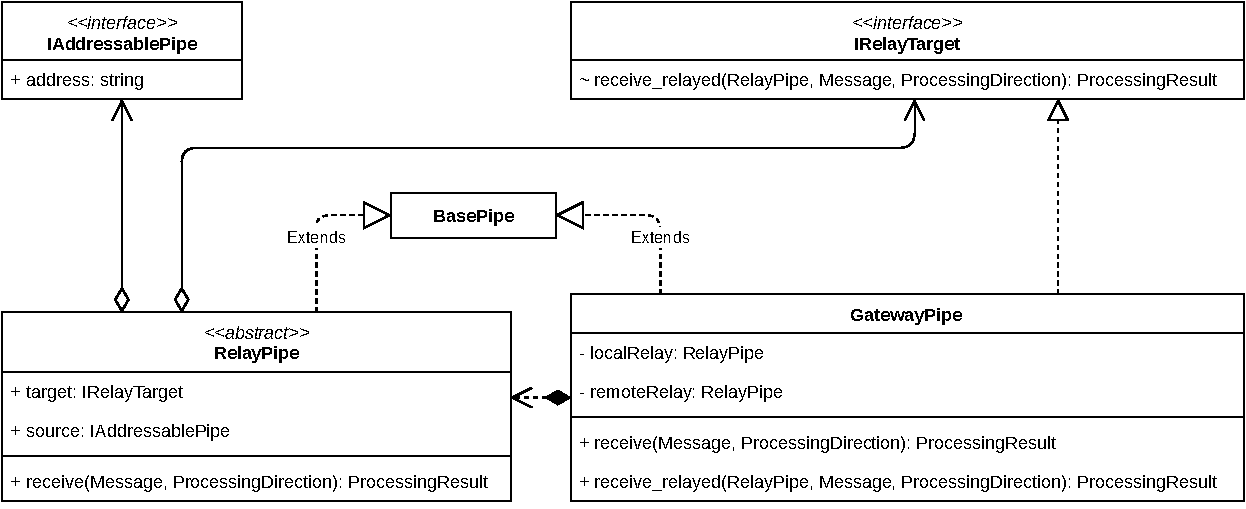
\includegraphics[width=14cm]{img/ch05/classes-3-gateway.pdf}
    \captionof{figure}{?} %TODO: Describe
    \label{fig:classes-3-gateway}
\end{figure}
\subsection{Gateway} The gateway component is defined by the \enquote{IGateway} interface shown in figure \ref{fig:classes-3-gateway}. It is designed to be run as a service in a separate thread that interacts with communication interfaces on machines (i.e. Bluetooth dongles or Ethernet interfaces). During operation it accepts incoming connections C\textsubscript{I} and creates its own respective outgoing connections C\textsubscript{O} to remote servers. Pairs of connections C\textsubscript{I} and C\textsubscript{O} are held in technology-specific pipe implementations and encapsulated in individual \enquote{RelayPipe} instances. Those RelayPipe instances are assigned to \enquote{GatewayPipe} instances. Improving on the first prototype's design, the GatewayPipe acts as a multiplexing pipe that accepts messages originating from the two encapsulating \enquote{RelayPipes} that act as two communication ports (e.g. the client device and the cloud server of scenario \#2 described in section \ref{sec:example-scenarios}) that hold information about the address of their communication peers in their address field (e.g. an \ac{IP} address of the remote peer). For instance, two \ac{TCP} client sockets can be handled by two \enquote{TcpPipes} (that inherit from the RelayPipe class), allowing \ac{TCP} packets to be routed into the pipeline via a GatewayPipe. Once messages are processed and sent back up the pipeline to a GatewayPipe, the GatewayPipe can find the correct RelayPipe to relay the message to by comparing their addresses with the message's \enquote{MessageDirection} information.


\begin{figure}[h]
    \centering
    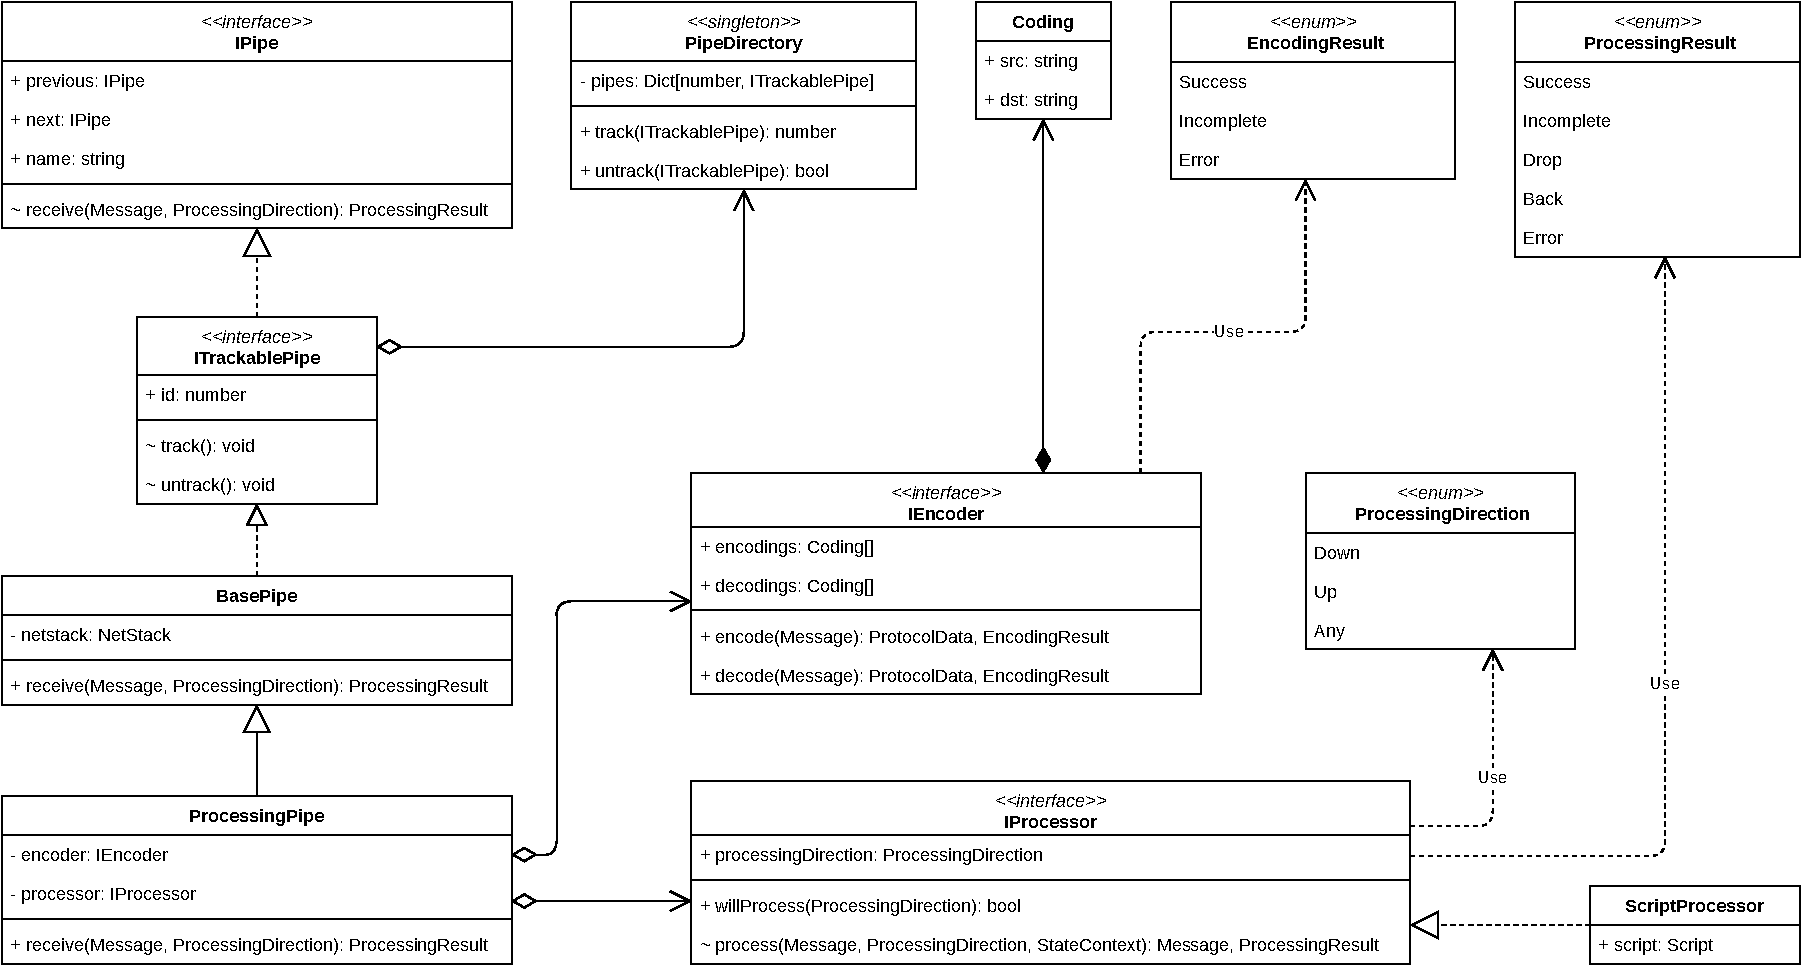
\includegraphics[width=14cm]{img/ch05/classes-2-pipes.pdf}
    \captionof{figure}{?} %TODO: Describe
    \label{fig:classes-2-pipes}
\end{figure}

\subsection{Pipes} Building upon the approach of routing and processing messages via pipes discussed in section \ref{sec:prototype-design}, this design concept addresses some inconsistencies of the former design and adds needed flexibility. As shown in figure \ref{fig:classes-2-pipes}\footnote{A larger printout \ref{fig:app-classes-2-pipes} can be found in the appendix.}, the \enquote{IPipe} interface is reused from the first prototype and extended by the \enquote{ITrackablePipe} interface that adds a unique identifier to pipes. This enables the application to easily locate pipes by looking up their identifiers in the \enquote{PipeDirectory}, allowing to interact with and inject messages into individual pipes directly.\\
A \enquote{BasePipe} implements the ITrackablePipe interface as well as simple routing logic for forwarding messages up and down pipelines. However, only \enquote{ProcessingPipes} actually perform any kind of operations on messages directly: they can employ \enquote{IEncoders} for (de-)serialization and \enquote{IProcessors} for transformation of messages. Contrary to the design concept of the first prototype, IEncoders need to specify which data formats they support as source and target encodings. This allows the implementation of multiple IEncoders for the same protocol that work with different source or target data formats. For example, some IEncoder may only provide decoding functionality for raw binary data into \ac{HTTP} messages with raw binary bodies while another implementation provides functionality to encode strings into \ac{HTTP} message bodies. In the first prototype's design, the very concept of filters was only vaguely described and lacked a clear and concise interface. This issue is resolved in this next iteration of the design concept:
\begin{itemize}
    \item Filters are renamed to \enquote{IProcessors} (conveying the purpose and meaning of the interface in its name).
    \item IProcessors specify a \enquote{ProcessingDirection} that determines whether messages shall be processed on their way \emph{down} or \emph{up} a pipeline or in any direction, effectively granting control over applying transformations on messages. This can be helpful when transformations shall only be applied in one direction or maybe only once in a pipeline, like replacing the contents of the body of an \ac{HTTP} message.
    \item An IProcessor can apply logic to messages in its \emph{process} method that also receives the pipeline's context. The returned \enquote{ProcessingResult} indicates success or failure of the operation or whether the IProcessor requests dropping a message or sending it back up the pipeline.
\end{itemize}
While there are many opportunities for specific implementations of the IProcessor interface, one general implementation is envisioned by the design concept: a simple \enquote{ScriptProcessor} allows penetration testers to supply scripts that are executed at runtime and allow transformation of messages. This directly fulfils the requirement \enquote{F5 Scripting}.
\begin{figure}[h]
    \centering
    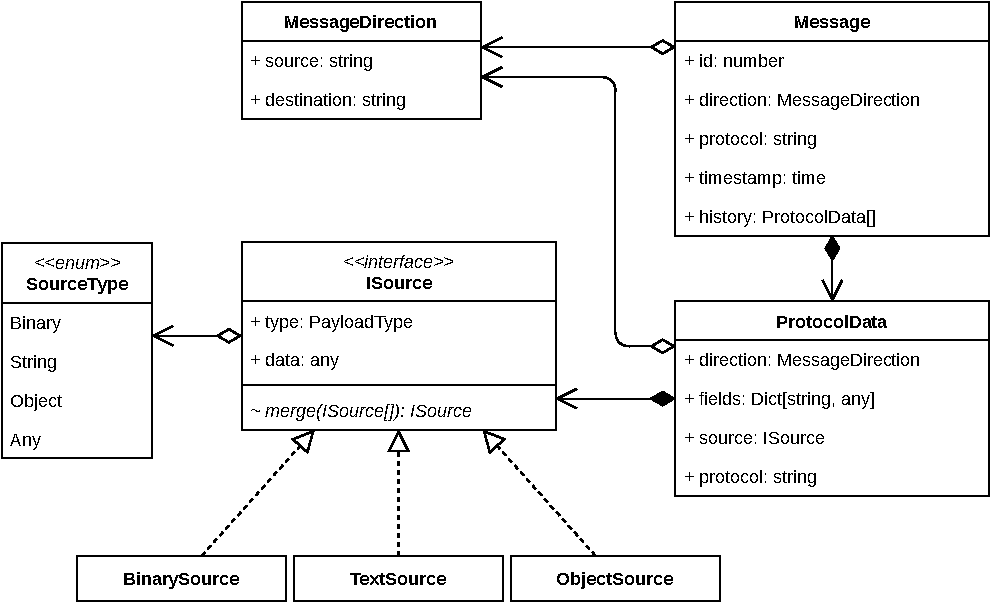
\includegraphics[width=14cm]{img/ch05/classes-4-messages.pdf}
    \captionof{figure}{?} %TODO: Describe
    \label{fig:classes-4-messages}
\end{figure} %TODO: Appendix!
\subsection{Messages}
Compared to the first prototype's design, the data-structures that represent messages are mostly unchanged (as shown in figure \ref{fig:classes-4-messages}). However, during implementation and testing of the first prototype it became apparent that in some cases \enquote{historical} information about messages was required. This iteration of the design adds a list of \enquote{ProtocolData} instances to messages that specify information about the protocol, message headers and the payload (\enquote{ISource}). IProcessors and IEncoders append newly transformed or (de-)serialized ProtocolData instances to messages. So over time, a message contains records of all those operations performed on it. This information can be useful in a number of cases like serialization: when a message is deserialized (e.g. the payload of a \ac{WS} message is extracted) on its way down a pipeline, important information about the formerly encapsulating protocol is lost (such as the \ac{WS} frame's flags). When a message is serialized on its way back up a pipeline, an IEncoder would have to generate this information or try and deduce it from the message, which is not always possible. However, since it can access the messages' history and former ProtocolData, it can read the original information and use this for serialization.

\section{Design \#2: Distributed Proxy Services}
\label{sec:design-2}
The design shown in section \ref{sec:design-1} was an iteration of the design worked out for the first prototype in section \ref{sec:prototype-design} and addressed some fundamental, architectural flaws and aimed for better flexibility and more meaningful interface definitions. However, it did not address other problems that were encountered during the implementation of the first prototype: constraints in platform, framework and programming language compatibility and flexibility. As a consequence of these constraints, the proxy application needed to be developed as a monolithic application. Therefore, each extension, like additional IEncoders that added support for new protocols, was required to be implemented in the same programming language and run on the same platform and as part of the same process as the proxy application. This also effectively limited the available selection of libraries. Another potential problem of the former design concept was the tight coupling of pipes and the deeply nested structure and hierarchy of state-machines, pipes and network stacks. While this architecture allowed to implement routing messages through composition (\emph{by design}), it greatly added to the runtime complexity and made debugging the application significantly harder.
\begin{figure}[h]
    \centering
    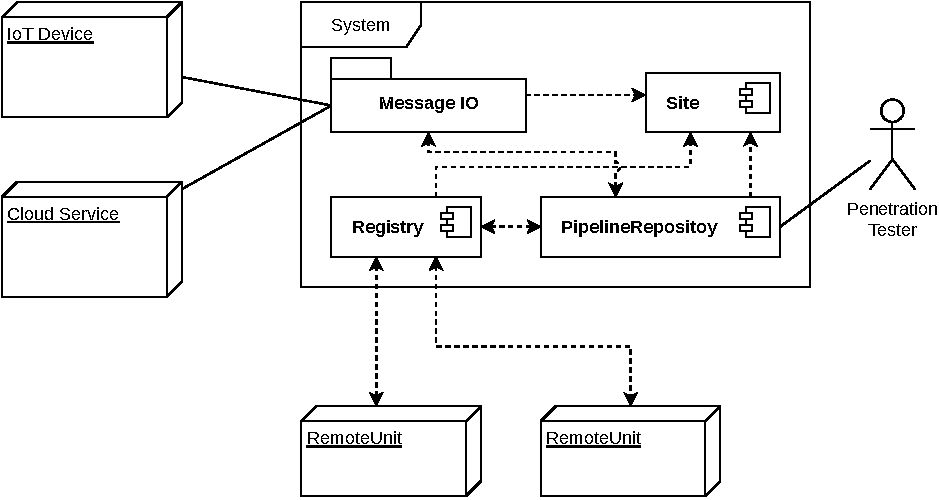
\includegraphics[width=14cm]{img/ch05/component-view2-1.pdf}
    \captionof{figure}{?} %TODO: Describe
    \label{fig:component-view2-1}
\end{figure}
\subsection{Overview}
Another iteration of the design (shown in figure \ref{fig:component-view2-1}) was made to address these issues. While the \enquote{Message IO} and \enquote{Site} components are left unchanged, the global state-machine is replaced by the \enquote{Registry} and \enquote{PipelineRepository} components that allow for de-centralized and more controlled processing of messages.

\begin{figure}[h]
    \centering
    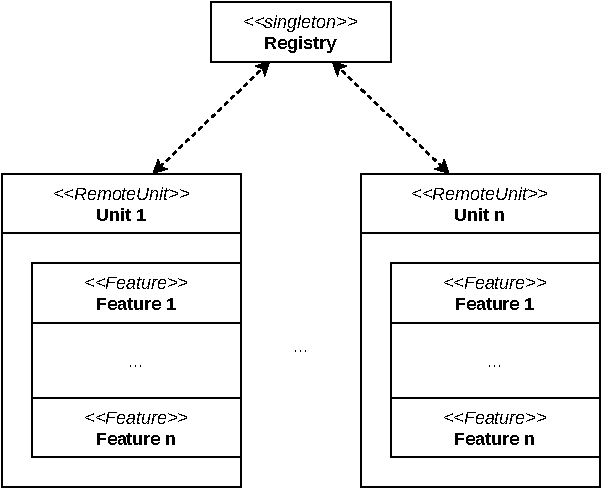
\includegraphics[width=10cm]{img/ch05/registry-remoteunit.pdf}
    \captionof{figure}{?} %TODO: Describe
    \label{fig:registry-units}
\end{figure}
\begin{figure}[ht]
    \centering
    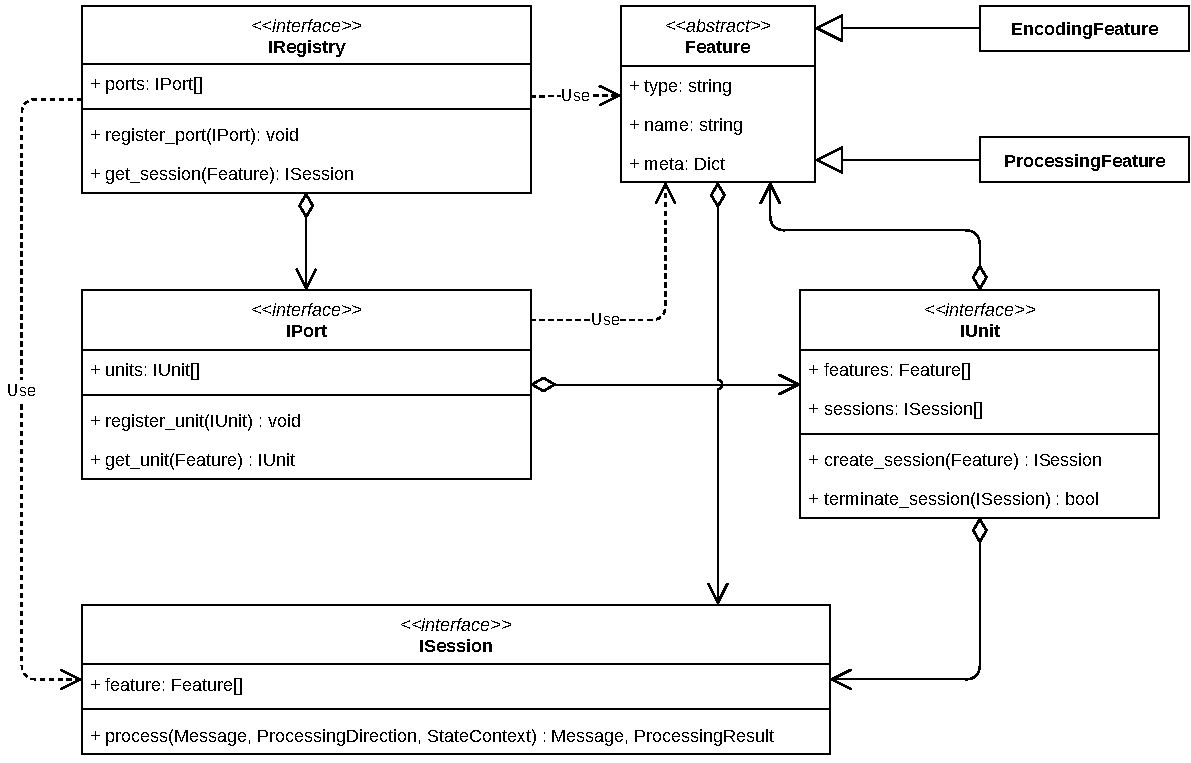
\includegraphics[width=14cm]{img/ch05/component-view2-3-registry-port-unit.pdf}
    \captionof{figure}{?} %TODO: Describe
    \label{fig:component-view2-3-registry-port-unit}
\end{figure}
\subsection{Registry and Units} To implement de-centralized processing of messages, a central registry is required to register remote units (shown in figure \ref{fig:registry-units}).
As can be seen in figure \ref{fig:component-view2-3-registry-port-unit}, the central registry is represented by the \enquote{IRegistry} interface that allows remote units to register themselves and allows the PipelineRepository to request sessions to units that implement requested features. Remote units can be remote machines that implement the \enquote{IPort} interface that provides a list of \enquote{IUnit} instances. An IUnit implements one or more \enquote{Features}, such as specific (de-)serialization or other processing, and effectively provides IEncoder and IProcessor functionalities. This transforms formerly direct calls to IEncoders and IProcessors to \acp{RPC}. Since IEncoders and IProcessors can be stateful, IUnits initialize them in \enquote{ISessions} for each requested feature. The IRegistry and IPort interfaces are explicitly kept rather simple and unspecific to the exact means of communication between them so that they can be implemented in various ways, making use of various \ac{IPC} techniques.\\
Also, to transmit data between the proxy application and its remote units, this data needs to be (de-)serialized and a format for serialization has to be chosen.

\subsection{PipelineRepository} The PipelineRepository component holds information about all configured pipelines (that is a flattened representation of the hierarchically configured state-machines and network stacks) and their contexts. This allows to remove the pipes from the software architecture, providing better traceability of messages throughout the system and makes debugging the high-level application logic more accessible. Also, organizing network stacks and state-machines in one central place encourages creation of means to interface with these mechanisms such as \ac{REST}-\acp{API} that let penetration testers inspect the message queue and ongoing processes.

\subsection{State of the Design Concept} This design concept promises to solve severe issues of the previous design iteration shown in section \ref{sec:design-1} and already defines some very high-level components. However, due to time constraints some components' designs were not  finished and require further work on specifics. For this, certain questions need to be answered and translated into the design:
\begin{itemize}
    \item \textbf{PipelineRepository:} How exactly is the hierarchy of state-machines and network stacks flattened? How is this flattened hierarchy represented in data-structures? How are instances of individual state-machines and network stacks initialized and organized for individual gateway-connections?
    \item \textbf{ISession:} How is information relevant to IEncoder and IProcessor instances (such as ScriptProcessors' Script instances) passed to remote units?
    \item \textbf{IRegistry/IPort:} How exactly are \acp{RPC} performed? Are there mature and appropriate frameworks that provide \acp{RPC} implementations?
\end{itemize}


\subsection{Comparison of Both Designs}
\label{sec:design-comparison}
Both design concepts discussed in the previous sections, the monolithic and the distributed concept, promise to solve specific problems. The following paragraphs compare both concepts on the base of a set of core design aspects:
\paragraph{Software architecture}
The monolithic concept suggests a centralized and self-contained design that combines the high-level business logic of a proxy-application with low-level tasks such as (de-)serialization of various protocols. It is designed to be run on a single machine.\\
In contrast to this, the distributed concept separates the high-level business logic (like routing messages) and low-level tasks as part of a client-server model: the high-level logic is implemented in the central proxy server while low-level tasks are isolated into separate remote services. These services can either be run on the same machine the proxy server runs on or on external machines. Through dynamic creation and registration of remote service instances, this concept also implements scalability. Since there is no restrictions to the programming languages, platforms or frameworks used by remote services, the concept also embraces platform compatibility.
\paragraph{Complexity}
The reliance on deeply nested data-structures has a high impact on the complexity of the monolithic concept at runtime. This makes debugging an implementation of this concept significantly harder and more time-consuming. However, adding new extensions to this concept becomes a comparatively easier task as integration of such new extensions only takes place on a source-code level.\\
As opposed to this, the distributed approach simplifies the high-level tasks such as routing messages by introducing distributed components that allow traceability and thus establish transparency. The offloading of protocol implementations into logical units that are accessed via \ac{IPC} however contribute to a more challenging deployment of the application. Also, due to their distributed nature, debugging these remote units can introduce further problems (e.g. connection losses and high latencies) and requires a more sophisticated and complex testing environment than the monolithic concept.

\paragraph{Maturity}
Some of the core components of the monolithic concept were already tested and proven by the first prototype. For instance, linked pipes proved to be an effective means to route and process messages up and down a processing pipeline. However, due to time-constraints, other core concepts such as the state-machines could not be tested. Regarding completeness, it is noteworthy that this concept's interfaces are well-defined.\\
Contrary to this, the distributed concept is not finished and requires further work to clear up a number of essential questions before it can be completed. Also, the previously proven effective idea of using pipes for routing and processing is removed in the distributed approach. This denies the approach any effectiveness acquired through previous design iterations.
% 5. Prototyp (Implementierung, Patterns, Tests)
\chapter{Implementing the Modular Proxy Application}
\label{chap:implementation}
This chapter covers an exemplaric implementation of the concept that was worked out in chapter \ref{chap:conceptual-design}, starting with formally describing the goals and constraints of this implementation in section \ref{sec:goals-constraints}. Afterwards, an overview and comparison of available and suitable tools for the task is performed in section \ref{sec:tool-selection}. The chapter concludes with details about the implementation of individual components in section \ref{sec:individual-components}, describing how specific challenges were overcome and what design patterns were used.

\section{Goals and Constraints}
\label{sec:goals-constraints}
\emph{TBD} %TODO: Write out
\begin{itemize}
    \item \emph{Focus on complex scenario \#2: HTTP, WS, MQTT}
    \item \emph{No interactive mode}
    \item \emph{Fully implement factories, state-machines and netstacks as POC}
\end{itemize}

\section{Tool Selection}
\label{sec:tool-selection}

\subsection{Requirements to the Tools}
\emph{TBD} %TODO: Write out
\begin{itemize}
    \item \emph{Scriptable!}
    \item \emph{Low-level access to APIs}
    \item \emph{Rich set of low-level libraries for protocol implementations}
    \item \emph{Accessible and easily extendable}
\end{itemize}

\subsection{Comparison of Programming Languages, Frameworks and Libraries}
\emph{TBD: Discuss how the candidates match the above-mentioned criteria and point out why python was chosen} %TODO: Write out
\begin{itemize}
    \item \emph{Native C: Win32 API / Linux ABI}
    \item \emph{.NET Visual C\# \& NuGet}
    \item \emph{JavaScript/TypeScript \& npm}
    \item \emph{Python \& pip}
\end{itemize}

\section{Individual Components}
\label{sec:individual-components}

\subsection{Network Stack}
\subsubsection{Gateways}
\subsubsection{Pipes, Encoders and Processors}
\subsubsection{Scripting}
\subsubsection{Pipelines}

\subsection{Finite State Machine}
\subsubsection{States}
\subsubsection{Transitions}
\subsubsection{Nested \acp{FSM}}

\subsection{Configuration Parsing and Building}
\subsubsection{Factories, Builders and Templates}
% 6. Post-Mortem 
\chapter{Evaluation}
\label{chap:evaluation}
This chapter attempts to identify and spell out the causes of the project failure. The project timeline will allow a quantitative overview of the project progression and show what parts of the project slowed down progress. Then, an overview of the qualitative aspects of the deliverables will discuss the maturity of the implementation and which parts reached a satisfactory level. %TODO: Restructure

\section{What Constitutes the Failure}
\emph{TBD: What failed? Why was the implementation not successful?}

\section{Quantitative Overview: Time Management}
\label{sec:pm-time-management}
Comparing the planned thesis schedule to the actual course it has taken, this section discusses how the intended plan was implemented and changed at certain places. Also, it will examine the causes of the delays during development.
\subsection{Project Timeline}
\label{sec:project-timeline}
Table \ref{fig:thesis-schedule} shows the initially planned thesis schedule divided into four phases, laying out the course of the thesis over a span of 24 weeks.

\begin{table}
    \centering
    \begin{tabular}{l l}
        \toprule
        Phase / Task             & Duration              \\
        \midrule
        1. Preparation           & $4$ weeks ($16,66\%$) \\
        \midrule
        Literature Research      & $1$ week              \\
        Expert Interviews        & $1$ week              \\
        Testbed Configuration    & $2$ weeks             \\
        \midrule
        2. Prototype             & $7$ weeks ($29,16\%$) \\
        \midrule
        Prototype Conception     & $2$ weeks             \\
        Prototype Implementation & $4$ weeks             \\
        Expert Feedback          & $1$ week              \\
        \midrule
        3. Functional Prototype  & $7$ weeks ($29,16\%$) \\
        \midrule
        FP Conception            & $2$ weeks             \\
        FP Implementation        & $4$ weeks             \\
        Expert Feedback          & $1$ week              \\
        \midrule
        4. Finalization          & $6$ weeks ($25\%$)    \\
        \midrule
        MQTT Case Study          & $2$ weeks             \\
        Thesis Finalization      & $4$ weeks             \\
        \midrule
        \midrule
        \emph{Total}             & \emph{$24$ weeks}     \\
        \bottomrule
    \end{tabular}
    \caption{Initially planned schedule for the thesis}
    \label{fig:thesis-schedule}
\end{table}

\paragraph{1. Preparation} The initial phase covered preparation tasks for further work on the thesis. Literature research on the topics covered and touched in this thesis was carried out. Related work on \ac{IoT} and \ac{ICS} security analysis (as discussed in chapter \ref{chap:related-work}) was of special interest as those showed what approaches had been taken to assess security implementations. Also, a testbed (discussed in section \ref{sec:prototype-testing}) for running the proxy application was built. A decision was made against conducting expert interviews before implementing a first prototype on the assumption that practical experience with the subject matter would benefit the expert interviews. The fact that a number of important questions arose from work on the first prototype later proved this decision to be correct. Performing the literature research and building a testbed was completed within the intended schedule of three weeks.
\paragraph{2. Prototype} In the second phase, the prototype discussed in section \ref{sec:prototypical-implementation} was designed and implemented in weekly sprints. Preceding these sprints, a rough design of the prototype's architecture and runtime behaviour was worked out in one week that would serve as a base for further design refinement and implementation in the sprints. These sprints ran for eight weeks in total: the initial design turned out to be too oversimplified so that sprints aiming to design and implement specific components were conducted rather isolated from other components that still needed to be worked on. As a result, both the integration of individual components and their interaction would fail and require redesigns and time-consuming adjustments to their implementation. Also, neither was the prototype mature enough to be used as a proxy application, nor was the resulting design and implementation clean enough to suggest putting further effort into working on them. After these eight sprints, work on this prototype was stopped and the expert interviews discussed in section \ref{sec:interviews} were prepared and conducted. It was found that the project was technically challenging and more complex than initially anticipated so the expert interviews were conducted to aid in re-engineering the design concept.

\paragraph{3. Functional Prototype} The third phase was intended to yield a design concept mature enough to both fulfil realistic requirements to a proxy application and be implemented. This was initiated by switching the technology stack from TypeScript to Python and re-designing and re-implementing large parts of the first prototype. In order to avoid the same mistake of refining a vague design concept and spending time adjusting the design and implementation to make them work, two weeks were spent on iterations of new design concepts discussed in chapter \ref{chap:conceptual-design}. These concepts did not only define single components but also interfaces that specified how those components interacted with each other, aiming for clear separation of components and high flexibility in implementation. Components of the prototype that were independent of the communication protocols used at runtime, such as NetStacks and \acp{FSM}, were implemented first over the span of four weeks. Then, implementations for supporting the \ac{HTTP}, \ac{WS} and \ac{MQTT} protocols followed over a span of another six weeks. Work on this prototype was stopped after those ten weeks as the technical difficulties discussed in section \ref{sec:pm-challenges} made estimations over the remaining time needed to finish the prototype both hard to make and rather unreliable.
\paragraph{4. Finalization} The final phase was intended to conduct a case study on how the proxy application would perform on scenario \# 2 from section \ref{sec:example-scenarios}. Tests were made to run the proxy application in the testbed shown in section \ref{sec:prototype-testing} which featured the same communication protocols that were used in scenario \# 2. However, the proxy application failed to reliably transmit or encode the messages sent between the \ac{MQTT} client and broker, thus resulting in a broken communication channel. The complex runtime behaviour and very time-consuming debugging of the proxy application (further elaborated on in section \ref{sec:pm-challenges}) lead to the decision to stop the project.

\begin{table}
    \centering
    \begin{tabular}{l l}
        \toprule
        Phase / Task             & Duration            \\
        \midrule
        1. Preparation           & $3$ weeks ($12\%$)  \\
        \midrule
        Literature Research      & 1 week              \\
        Testbed Configuration    & 2 weeks             \\
        \midrule
        2. TypeScript Prototype  & $10$ weeks ($40\%$) \\
        \midrule
        Prototype Conception     & 1 week              \\
        Prototype Implementation & 8 weeks             \\
        Expert Interviews        & 1 week              \\
        \midrule
        3. Python Candidate      & $12$ weeks ($48\%$) \\
        \midrule
        RC Conception            & 2 weeks             \\
        RC Implementation        & 10 weeks            \\
        \midrule
        \midrule
        \emph{Total}             & \emph{25 weeks}     \\
        \bottomrule
    \end{tabular}
    \caption{Actual schedule of the project}
    \label{fig:thesis-schedule-actual}
\end{table}

Table \ref{fig:thesis-schedule-actual} shows the actual schedule of the thesis. As can be seen, $88\%$ ($22$ weeks) of the time working on the thesis was spent designing and implementing the prototypes compared to a planned portion of roughly $60\%$ ($14$ weeks).

% Typescript prototype: March 2020
% Python prototype: November 2020 - December 2020

\subsection{Development Challenges}
\label{sec:pm-challenges}
There was a series of development challenges that slowed down implementation of both prototypes considerably:
\paragraph{Complex runtime behaviour} The combination of nested \acp{FSM} and pipelines lead to several problems during development. Even comparatively simple scenarios to use the proxy application in required a complete configuration file. This file was made of a global state machine and at least one network stack. This lead to a dynamic and long chain of references at runtime that made tracing back calls and attributing them to specific instances difficult.\\
Some problems such as a timing problem in the implementation of \acp{FSM} were very time consuming to debug: an \ac{FSM} would change its state when any of its rules was evaluated successfully and indicated a state change. By design, all \acp{FSM} of an active netstack would evaluate their rules when a message entered or left any netstack. When a higher-level \ac{FSM} (e.g. the global state-machine) changed its state \emph{while} a message was still being processed in a lower-level \ac{FSM}, the higher-level state-machine would change to another netstack, thus disconnect the lower-level state-machine. Eventually, the message would be processed back up and run into a pipe that had no upstream connection anymore, raising an exception and terminating the program. This particular error was discovered during the implementation and testing of the \ac{MQTT} encoder, in a runtime setup that involved a global default state-machine with a default \ac{TCP} netstack and a state-machine that handled \ac{HTTP} to \ac{WS} upgrades and processed \ac{MQTT} messages utilizing network stacks for \ac{HTTP} and \ac{WS}/\ac{MQTT}.\\
Other problems uncovered design flaws and required prompt changes to the software design or, in some cases, introduced new constraints to the project. One such example was discovered while testing the \ac{HTTP} encoder implementation using Mozilla FireFox as an \ac{HTTP} client. When browsing websites, the browser would open multiple connections to the target host to acquire multiple files at the same time\footnote{For testing single \ac{HTTP} connections, the key \emph{network.http.max-connections-per-server} could be set to $1$ in the \emph{about:config} page.}. This required the proxy application to instantiate a new pipeline per incoming connection rather than reside on using a single pipeline. However, the pipeline design dictated that pipes were connected to at most one preceding and one succeeding pipe. In order to connect pipelines to \acp{FSM}, the \acp{FSM} needed to provide a pipe-interface themselves. Thus, when instantiating multiple pipelines, these could not be connected to the global state-machine because the global state-machine's pipe-interface could only be connected to a single pipeline at a time. Therefore, a multiplexing pipe needed to be implemented to solve this issue. Alternatively, the proxy application could enforce instantiation of one single pipeline only to avoid changes to the software design. For a lab environment, enforcing the use of a single connection might work, however in real scenarios this constraint could potentially lead to the proxy application breaking applications at runtime.
To enable future implementations to support multiple connections, the software design was changed in a way that would allow the proxy to handle multiple connections. However, due to its academic nature, the prototype would only support a single connection at a time to reduce complexity.
\paragraph{Open source libraries} Both prototypes made use of open source libraries that implemented various protocols and included serialization and de-serialization routines for handling protocol specific packets. However, such libraries appeared to be intended to be used for developing applications that used those protocols as a means for transporting data rather than directly parsing packets.\\
Usually, these libraries would offer an API that allowed to instantiate and operate clients and servers and bind callbacks to events. The implementations of packet serialization and de-serialization were often times hidden through encapsulation, missing typings or poorly documented. For instance, the JavaScript library \enquote{ws}\footnote{https://github.com/websockets/ws, version 7.0.0, commit 092a822a41eb22f6d6745c18bc29b9c40715680f} provided methods for serialization and de-serialization but lacked typings
%\footnote{The version used for the TypeScript prototype was version 7.0.0, source code is available at https://github.com/websockets/ws.}
. Typings for this library were made available by the project \enquote{DefinitelyTyped}, however those did not include the classes relevant for serialization and de-serialization (\enquote{Sender} and \enquote{Receiver})\footnote{https://github.com/DefinitelyTyped/DefinitelyTyped/, commit 4bf23527293b2943c7fc12585c21473905a564d7}
%\footnote{As can be seen here: https://github.com/DefinitelyTyped/DefinitelyTyped/blob/4bf23527293b2943c7fc12585c21473905a564d7/types/ws/index.d.ts}
.
At the time of implementing the Python prototype, it used the library \enquote{websockets} that offered only an async de-serialization method
%\footnote{The python prototype used the library at commit 6b5cbaf41cdbc9a2074e357ccc613ef25517dd32: https://github.com/aaugustin/websockets/blob/6b5cbaf41cdbc9a2074e357ccc613ef25517dd32/src/websockets/framing.py}
(\enquote{framing.Frame.read}), requiring the use of asyncio which was circumvented by implementing a wrapper around it.\\
The Python prototype also used the \enquote{hbmqtt} library to (de-)serialize \ac{MQTT} messages. The library used an object-oriented implementation for (de-)serializing \ac{MQTT} messages where a class for each \ac{MQTT} message type (e.g. \emph{CONNECT}, \emph{CONNACK...}) inherited from an abstract \enquote{MQTTPacket} superclass %\footnote{https://github.com/beerfactory/hbmqtt/blob/31165fb0e827925417f99a7b1f475a9d67e1c72f/hbmqtt/mqtt/packet.py\#L186}
that defined a \enquote{to\_bytes} method for serialization and an async \enquote{from\_stream} method for de-serialization. Since the library did not implement a generic method that parsed a byte-buffer and returned the appropriate \ac{MQTT} message object, this logic had to be implemented as part of the work in the prototype, requiring investigation of the (largely uncommented) source code of the library as its documentation did not cover these internal (de-)serialization methods but focused on high-level use of the API it implemented.\\
From a software engineering point of view, omitting public interfaces to internal (de-)serialization methods and forcing specific programming patterns (such as async programming) are perfectly valid decisions in the context of single, individual modules. However, for those reasons, making use of the functionalities implemented in those libraries, was not trivial. It involved developing workarounds and investigating the libraries' source code which in turn took up time during the implementation phases.\\
Then there were also instances of incomplete documentation: the Python library \enquote{websockets} implemented (de-)serialization of \ac{WS} packets and also implemented the \ac{PMCE}%\footnote{Available at https://github.com/aaugustin/websockets/blob/6b5cbaf41cdbc9a2074e357ccc613ef25517dd32/src/websockets/extensions/permessage\_deflate.py}
of the \ac{WS} protocol. Calling the (de-)serialization methods of the \enquote{websockets} library and specifying the use of \ac{PMCE}, the first incoming and outgoing messages would be compressed correctly, however following messages would be compressed incorrectly. This rendered the prototype useless as \ac{WS} may use \ac{PMCE} by default to reduce bandwidth. The library failed to raise exceptions or return error codes so from the prototype's runtime point of view it appeared to work just fine. After investigating the library's source code it was found that the instances implementing the extension were stateful. When supplying newly created instances of said extension implementation to the (de-)serialization methods, they worked as intended, compressing and decompressing any amount of \ac{WS} packets. This could be due to a multitude of reasons including improper use of the \ac{PMCE} instances or improper calling of the (de-)serialization methods. No documentation could be found about specifics on those specific topics, though.\\
For Python libraries, one reason why documentation was in some cases sparse, only documented high-level features and largely omitted in-code documentation (such as comments) might be the \enquote{pythonic} approach to writing Python code. \enquote{Pythonic} code values readability higher than performance and encourages writing self-explanatory code%TODO: ref https://dl.acm.org/doi/abs/10.1145/3276954.3276960
. While this way of programming may help to understand individual methods or even algorithms that use multiple methods, it does not by itself aid in documentation of high-level concepts or complex interaction. Another reason for sparse documentation in open source libraries might be the developers' focus on implementing more features or improving the code-base instead of aiming for more complete documentation. Contrary to commercial products, there usually are no monetary incentives for developers of open source software to write documentation.

\section{Qualitative: Deliverables}
\label{sec:pm-deliverables}
\emph{TBD: Which fit-criteria were met? What is the implementation currently capable of? Which requirements were not full-filled?}
% 7. Zusammenfassung
\chapter{Summary}
\label{chap:summary}
This chapter provides a summary of the concept shown in chapter \ref{chap:conceptual-design} and the implementation thereof in chapter \ref{chap:implementation}.

\section{Requirements Engineering}
\label{sec:summary-requirements-engineering}

\section{Concept}
\label{sec:summary-concept}
\emph{TBD:}
\begin{itemize}
    \item \emph{Pipelines + \acp{FSM} lead to tricky debugging. Decouple them and introduce a queue (+metadata) per connection.}
\end{itemize}

\section{Implementation}
\label{sec:summary-implementation}

\begin{figure}[h]
    \centering
    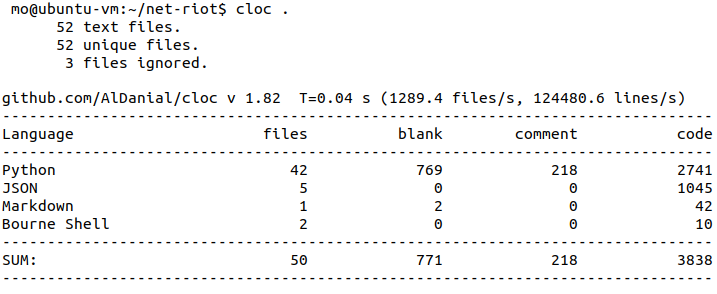
\includegraphics[width=12cm]{img/ch06/cloc.png}
    \captionof{figure}{?} %TODO: Describe
    \label{fig:cloc}
\end{figure}
\emph{TBD:}
\begin{itemize}
    \item \emph{Discuss technical debt!}
    \item \emph{Large config files: bad usability, also confusing}
\end{itemize}
% 8. Ausblick + Fazit
\chapter{Conclusion}
\label{chap:conclusion}

\emph{TBD}

\label{lastpage}

\cleardoublepage

\singlespacing

\pagenumbering{roman}
\setcounter{page}{\value{frontmatterpage}}

\addchap{\hsmaabbreviations}
\begin{acronym}[IEEE]
    \acro{A/C}{air conditioner}
    \acro{AP}{access point}
    \acro{API}{application programming interface}
    \acro{ARP}{Address Resolution Protocol}
    \acro{AWS}{Amazon Web Services}
    \acro{ENISA}{European Union Agency for Cybersecurity}
    \acro{FSM}{finite-state machine}
    \acro{GDPR}{General Data Protection Regulation}
    \acro{HMI}{human-machine interface}
    \acro{HTTP}{Hypertext Transfer Protocol}
    \acro{ICS}{industrial control system}
    \acro{IDE}{integrated development environment}
    \acro{IIoT}{Industrial internet of things}
    \acro{IoT}{Internet of things}
    \acro{IP}{Internet Protocol}
    \acro{IPC}{inter-process communication}
    \acro{ISP}{Internet Service Provider}
    \acro{JSON}{JavaScript object notation}
    \acro{MITM}{man-in-the-middle}
    \acro{MQTT}{message queuing telemetry transport}
    \acro{MTU}{maximum transmission unit}
    \acro{NAT}{Network Address Translation}
    \acro{OPC U/A}{OPC Unified Architecture}
    \acro{OT}{Operational Technology}
    \acro{PLC}{programmable logic controller}
    \acro{PyPI}{Python Package Index}
    \acro{PMCE}{Per-Message Compression Extension}
    \acro{QoS}{Quality of Service}
    \acro{REST}{Representational State Transfer}
    \acro{RPC}{remote procedure call}
    \acro{SSL}{Secure Socket Layer}
    \acro{TCP}{Transmission Control Protocol}
    \acro{TLS}{Transport Layer Security}
    \acro{UDP}{User Datagram Protocol}
    \acro{WS}{WebSockets}
\end{acronym}

\cleardoublepage
\phantomsection
\addcontentsline{toc}{chapter}{\hsmalistoftables}
\listoftables

\cleardoublepage
\phantomsection
\addcontentsline{toc}{chapter}{\hsmalistoffigures}
\listoffigures

\cleardoublepage
\phantomsection
\addcontentsline{toc}{chapter}{\hsmalistings}
\lstlistoflistings

\begingroup
\cleardoublepage
\begin{flushleft}
\let\clearpage\relax 
\printbibliography
\end{flushleft}
\endgroup

\cleardoublepage
\phantomsection
\addcontentsline{toc}{chapter}{\hsmaindex}
\printindex

\appendix
\chapter{Diagrams}


\begin{figure}[t]
    \centering
    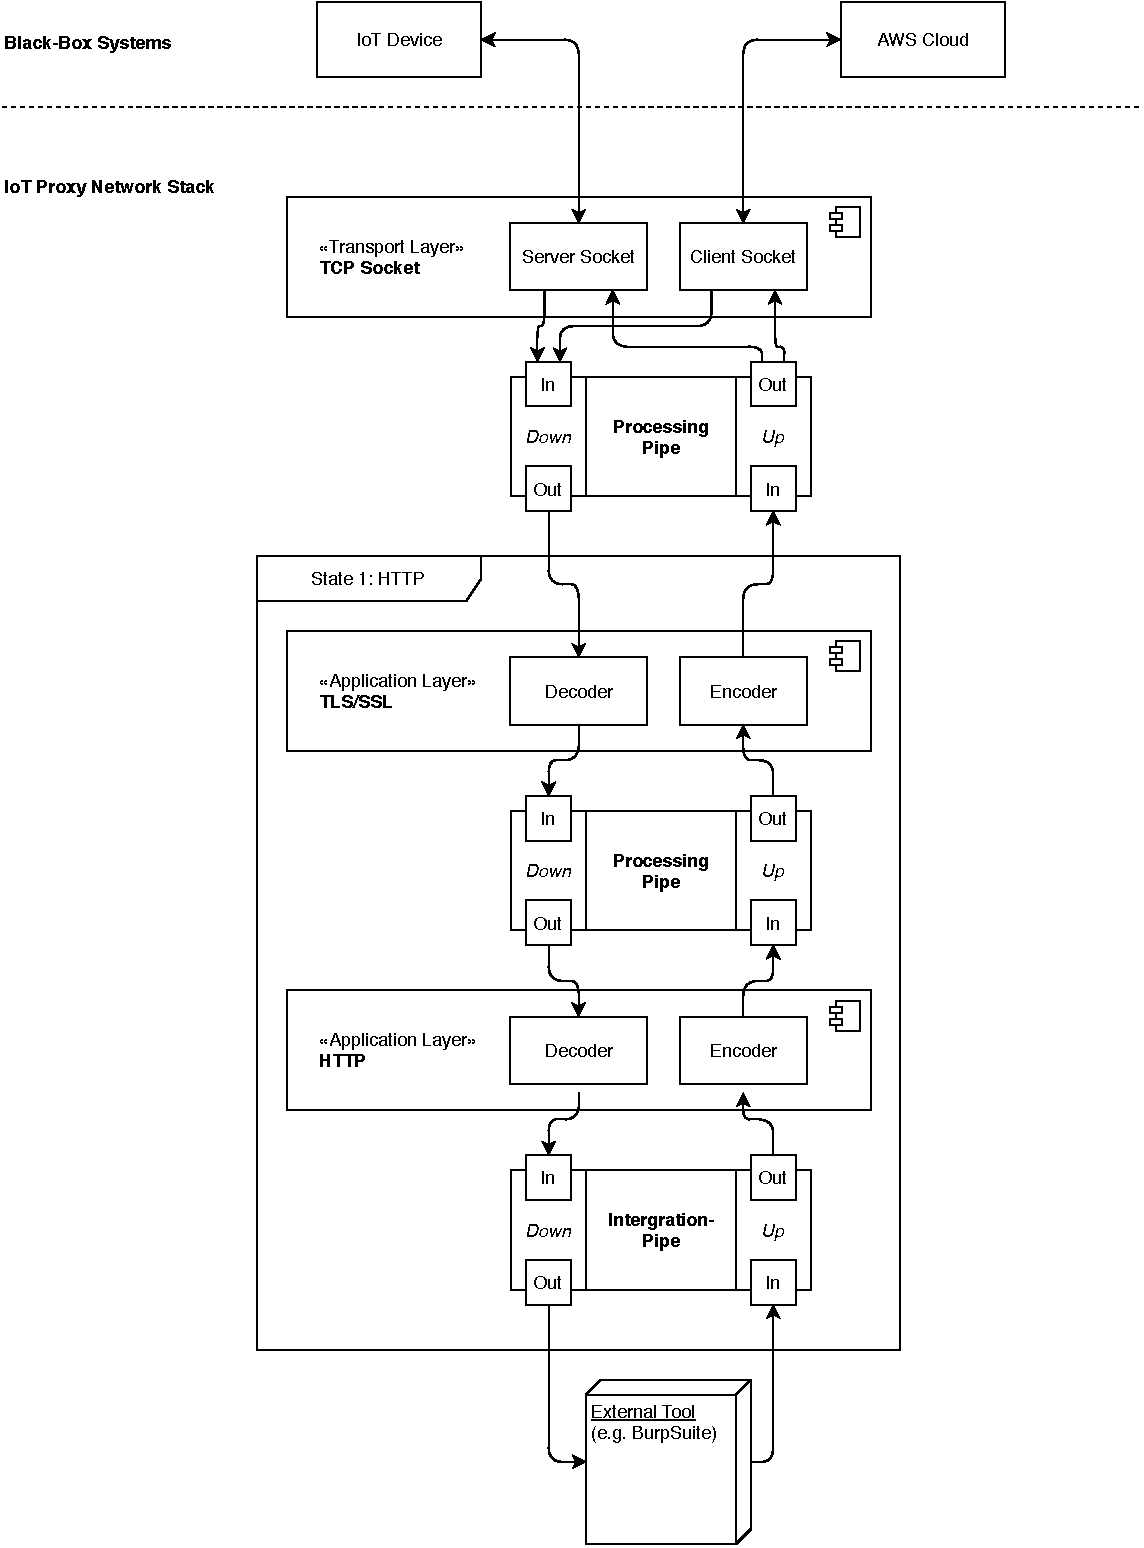
\includegraphics[width=14cm]{img/ch04/Architecture - PipesFilters 1.pdf}
    \captionof{figure}{\ac{AWS} \ac{IoT} Scenario - State 1: \ac{HTTP} Server}
    \label{fig:app-diag-pipesfilters-1}
\end{figure}

\begin{figure}[t]
    \centering
    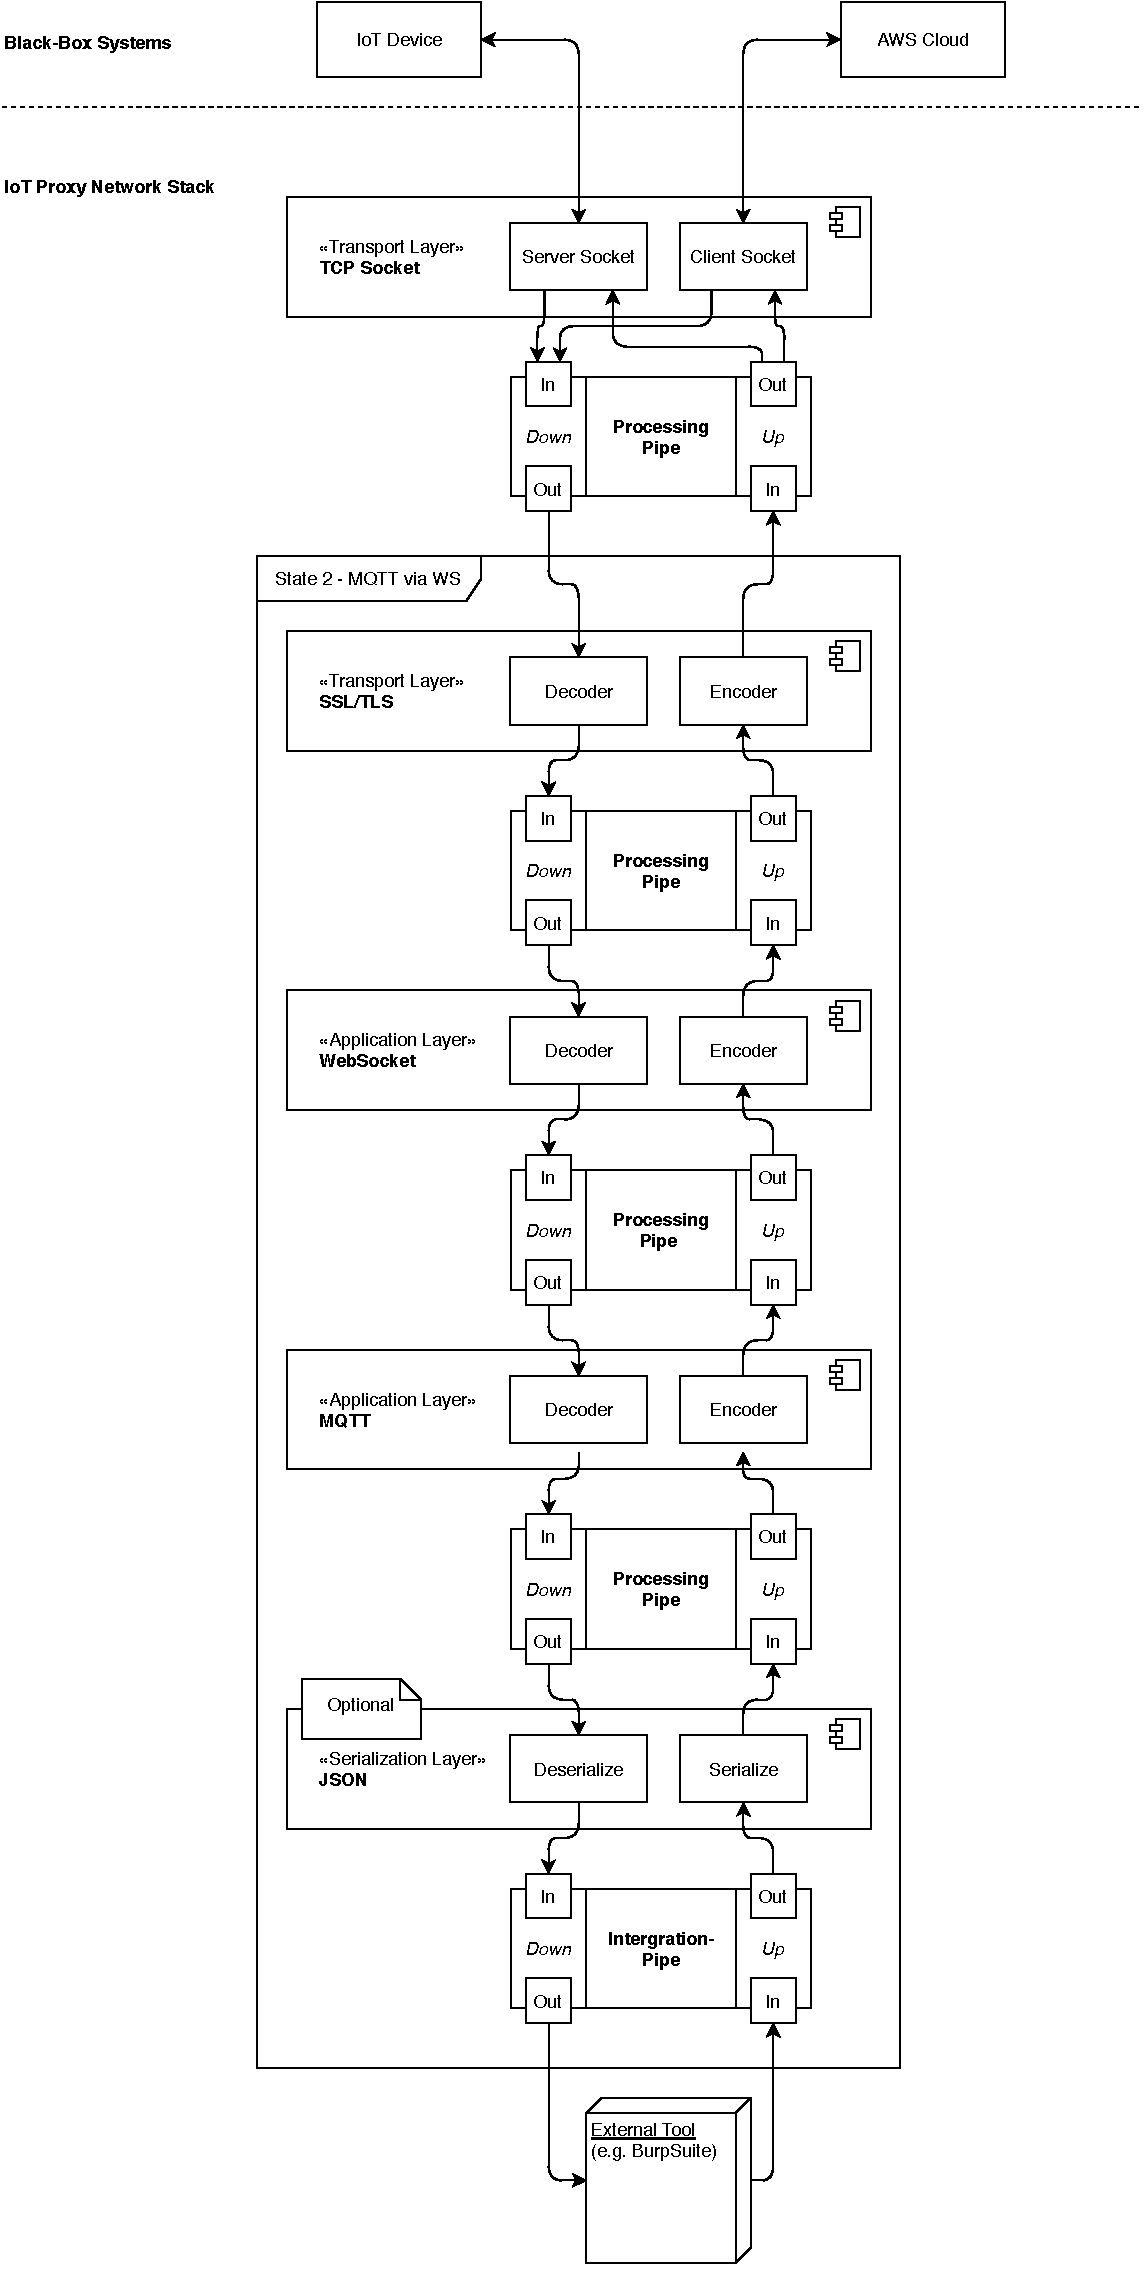
\includegraphics[width=12cm]{img/ch04/Architecture - PipesFilters 2.pdf}
    \captionof{figure}{\ac{AWS} \ac{IoT} Scenario - State 2: \ac{MQTT} via \ac{WS}}
    \label{fig:app-diag-pipesfilters-2}
\end{figure}

\begin{figure}[t]
    \centering
    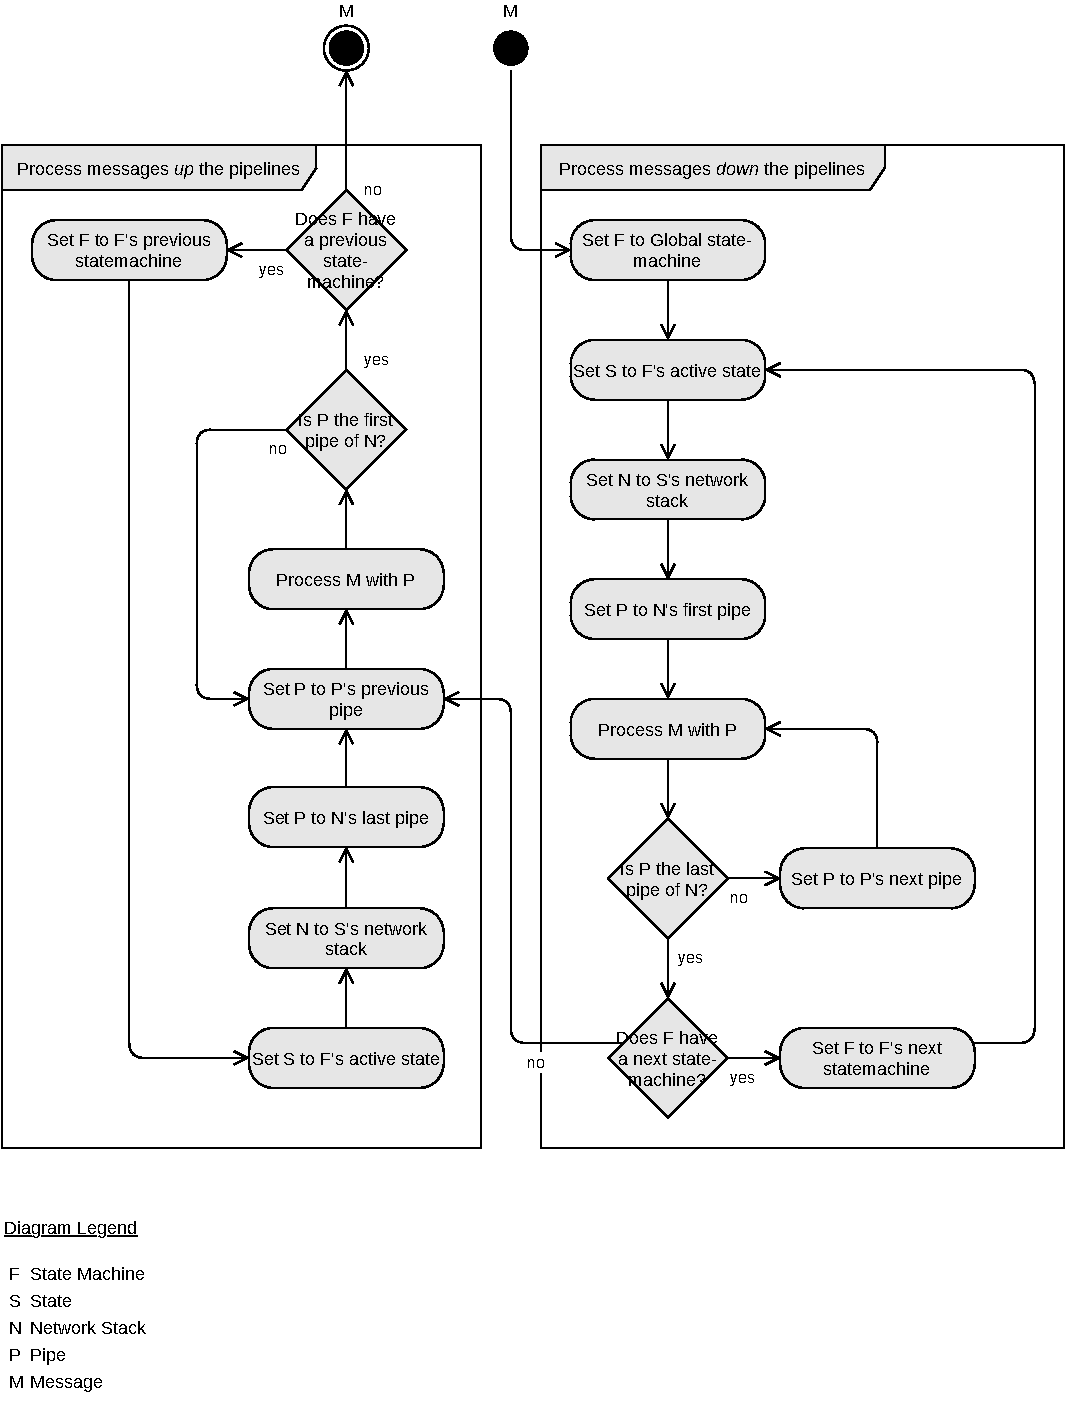
\includegraphics[width=14cm]{img/ch05/activity-nested-fsms.pdf}
    \captionof{figure}{Message processing through an architecture of nested \acp{FSM} and network stacks}
    \label{fig:app-activity-fsms}
\end{figure}

\begin{sidewaysfigure}[h]
    \centering
    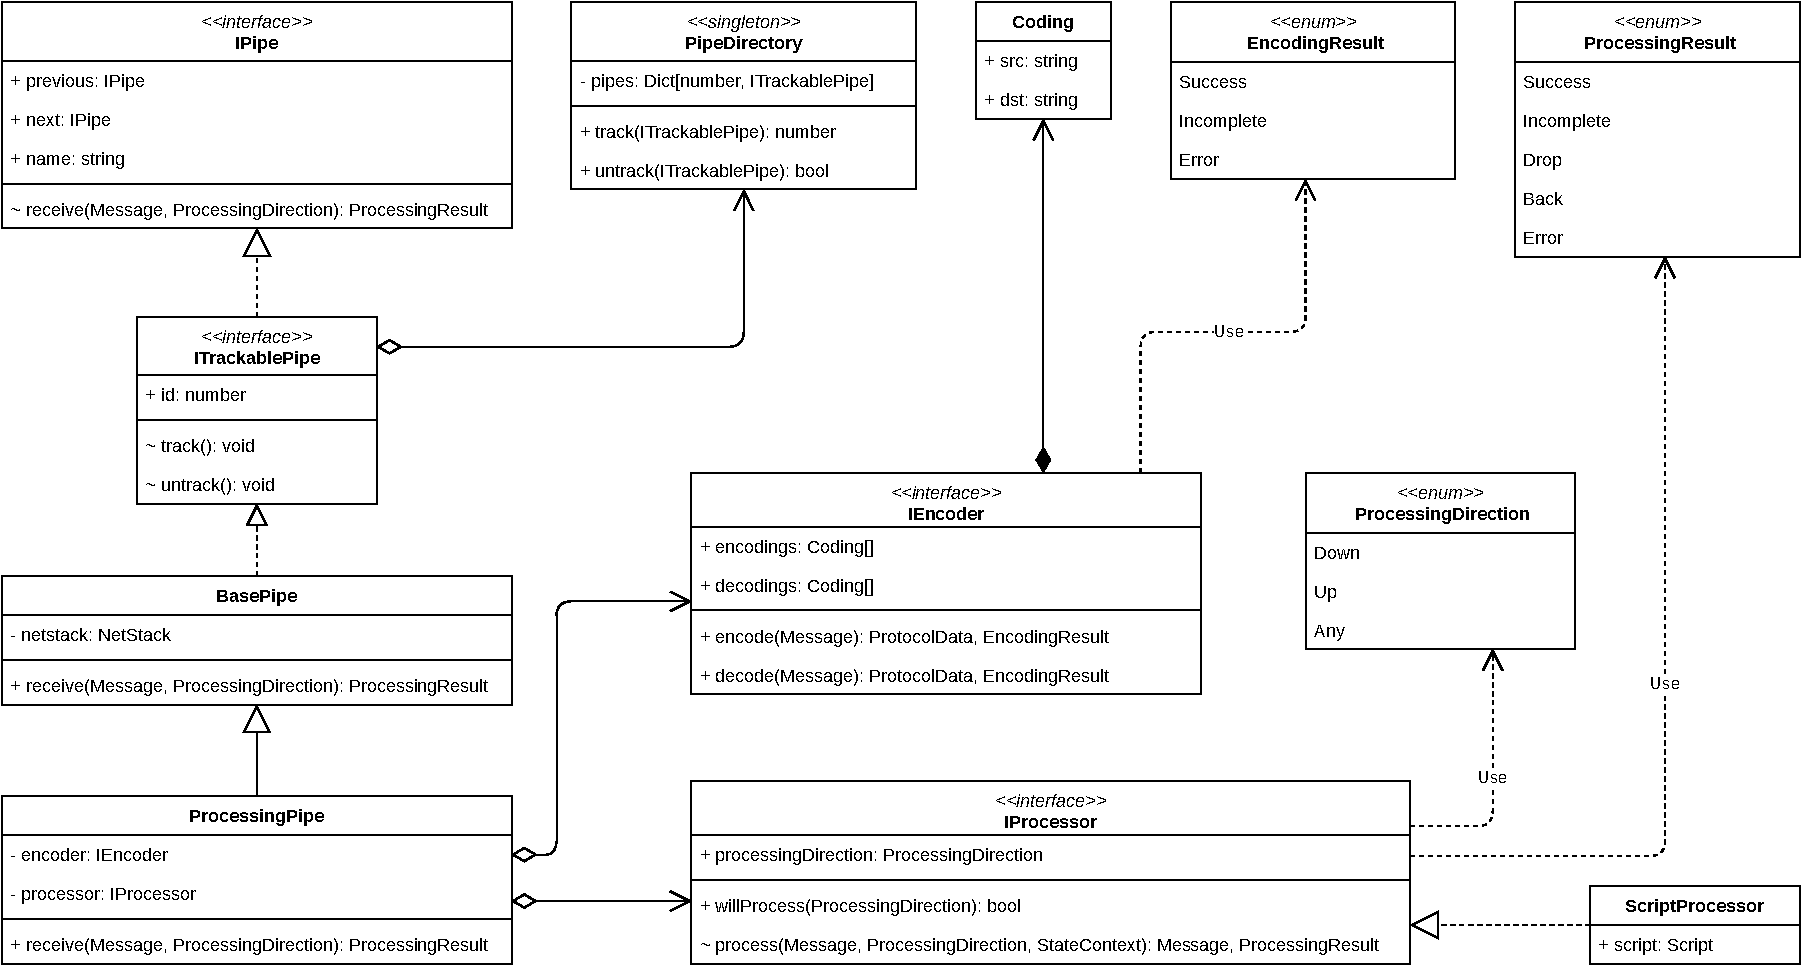
\includegraphics[height=12cm]{img/ch05/classes-2-pipes.pdf}
    \captionof{figure}{?} %TODO: Describe
    \label{fig:app-classes-2-pipes}
\end{sidewaysfigure}

\begin{figure}[h]
    \centering
    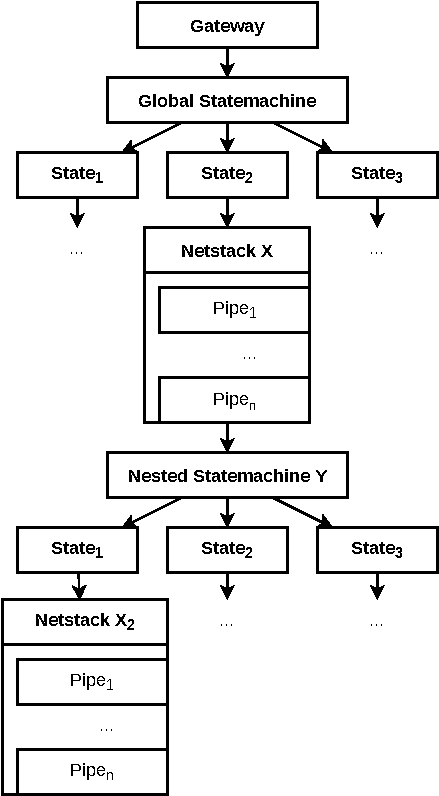
\includegraphics[height=12cm]{img/ch05/pipeline.pdf}
    \captionof{figure}{?} %TODO: Describe
    \label{fig:pipeline}
\end{figure}
%\chapter{Erster Anhang}

Hier ein Beispiel für einen Anhang. Der Anhang kann genauso in Kapitel und Unterkapitel unterteilt werden, wie die anderen Teile der Arbeit auch.

%\chapter{Zweiter Anhang}

Hier noch ein Beispiel für einen Anhang.


\end{document}
